\section{The ``M'' Problems}


\setcounter{page}{1}
\renewcommand{\thepage}{M-\arabic{page}}


%\renewcounter{Exercise}[subsection]
\counterwithin{Exercise}{subsection}
\renewcommand{\theExercise}{{\thesubsection}\arabic{Exercise}}
%\renewcommand{\ExerciseHeaderNB}{M\Alph{\subsection}\arabic{\Exercise}}
%\renewcommand{\ExerciseHeader}{\textbf{M\Alph{subsection}\ExerciseHeaderNB.\ExerciseHeaderDifficulty}}
\renewcommand{\ExerciseHeaderNB}{\thesubsection\arabic{Exercise}}
\renewcommand{\ExerciseHeader}{\textbf{\ExerciseHeaderNB.\ExerciseHeaderDifficulty}}
\renewcommand{\AnswerHeader}{\textbf{\ExerciseHeaderNB.} }
%\setlength{\AnswerSkipBefore}{0pt}
%\setlength{\AnswerSkipAfter}{0pt}
\setlength\Exerightmargin{3in}
\renewcommand{\AtBeginAnswer}{\setlength\Exerightmargin{3in}\hangindent=0.7cm}

%\numberwithin{Exercise}{subsection}

\titleformat{\subsection}{\normalfont\large\bfseries}{\thesubsection~Problems:}{1ex}{}

%\renewcommand{\sectionmark}[1]{\markboth{\MakeUppercase{\thesection:\ #1}}{}}
\renewcommand{\subsectionmark}[1]{
   \markright{\thesubsection~Problems: #1}}

\subsection{The Basics} 

%\DTMnewdatestyle{dateupdated}{〈definition 〉

Answers to M\Alph{subsection} problems are on page \pageref{the_basics_prob_answers}.  \textbf{\textcolor{red}{Updated \DTMnow.}}

%--------------------------------------------------------------------------------------------------------------
\begin{Exercise}[difficulty=1]
If you haven't done so already, please read the following documents on Blackboard under ``Course Information:''
\begin{itemize}[nosep]
\item The Syllabus
\item ``On Working Together Honestly''
\item About Lab Notebooks
\item Why no equation sheets
\end{itemize}
(a)~If you could change any aspect of these course policies (or anything else about the course, I guess), what would you change?  You must make at least one suggestion for a change; no fair just answering that you're fine with whatever's currently there.  (b)~How serious are you about this request?  (Are you just suggesting a change because it was required, or because you genuinely think it would improve the course?)
\end{Exercise}

%--------------------------------------------------------------------------------------------------------------
\begin{minipage}{0.7\textwidth}
\begin{Exercise}
A student wants to find the internal resistance of a standard, size-AA battery.  With no load resistor connected, the voltage across the terminals of the battery is 1.55~V.  But when the battery is connected to a load resistor of 10~$\Omega$ (as shown on the right) the voltage across the load resistor is 1.47~V.  What is the internal resistance of the battery?
\end{Exercise}
\begin{Answer}
0.544~$\Omega$ The circuit is built correctly and the output is within the range expected for the tolerances of the components. The circuit is built correctly and the output is within the range expected for the tolerances of the components. The circuit is built correctly and the output is within the range expected for the tolerances of the components.
\end{Answer}
\end{minipage}
\begin{minipage}{0.30\textwidth - 5pt}
\hfill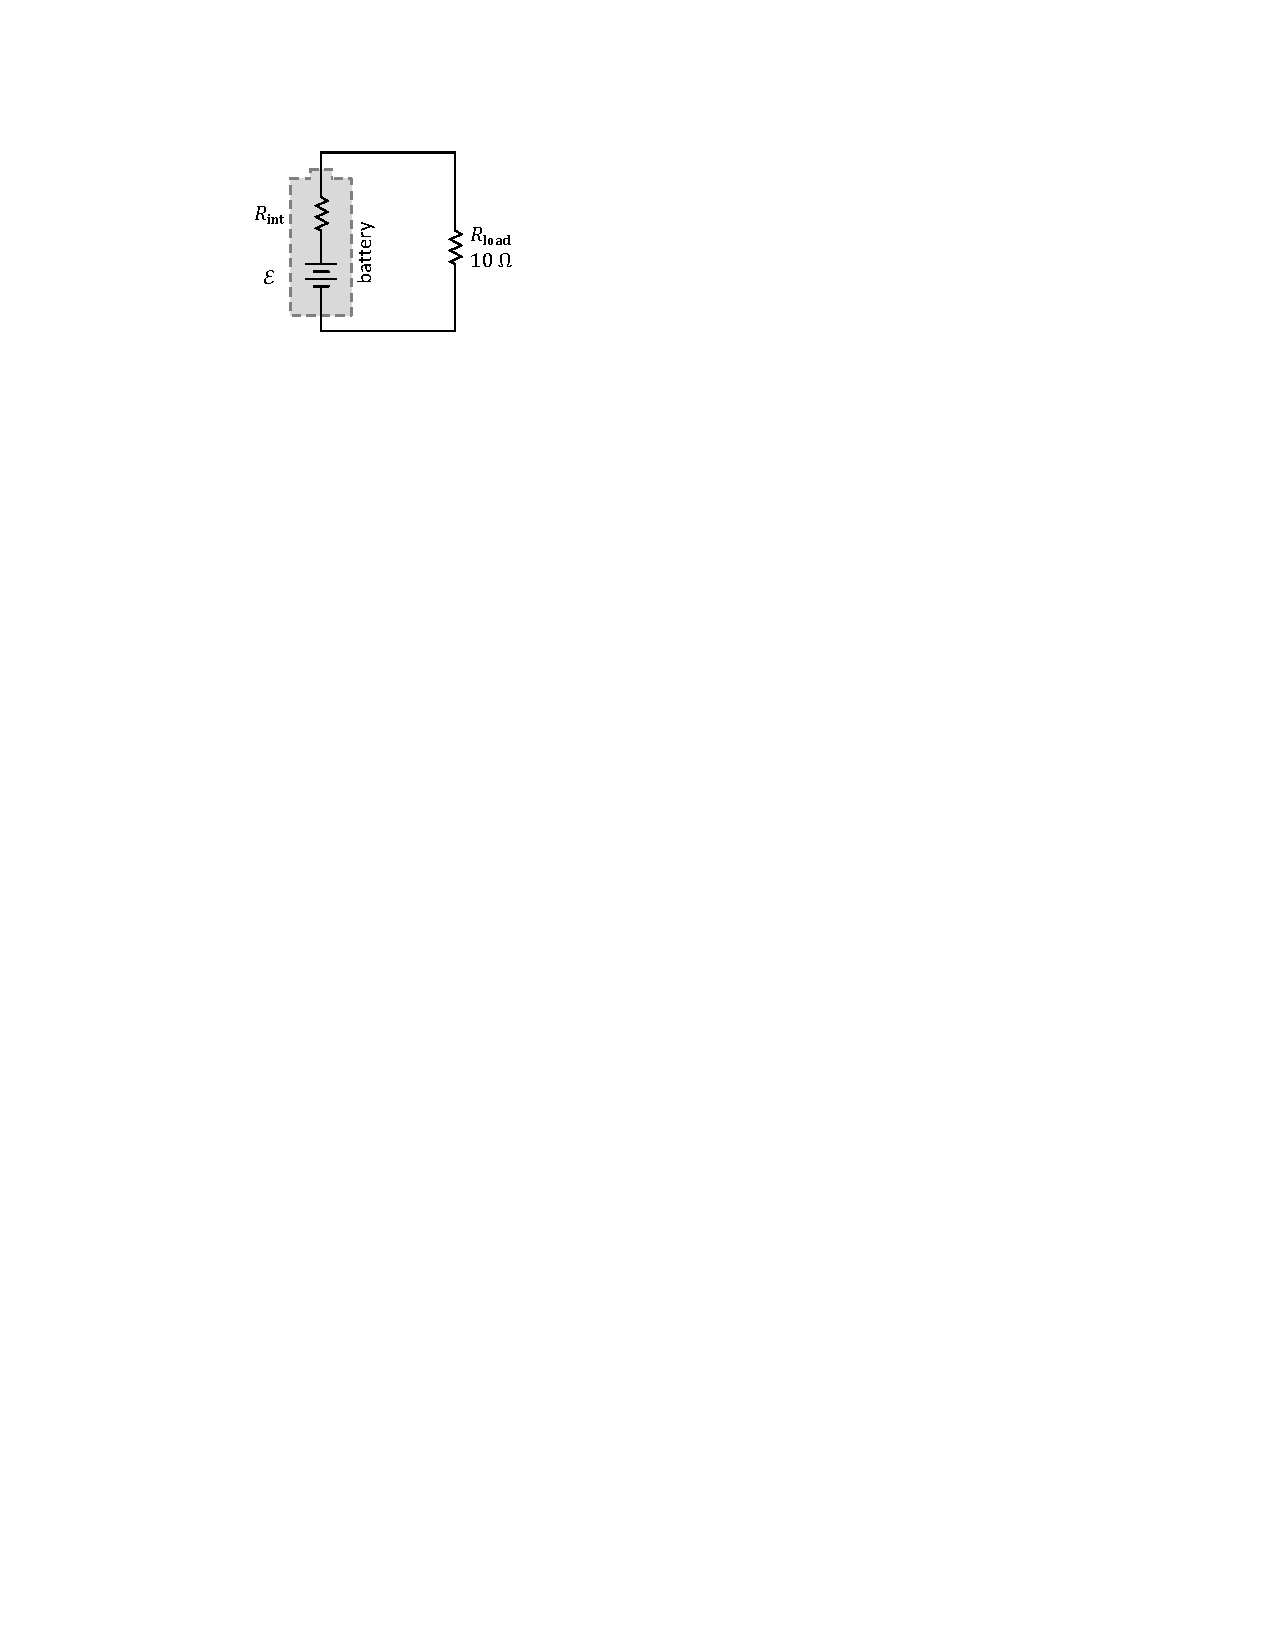
\includegraphics{M_problems/the_basics/real_battery_10ohms.pdf}
\end{minipage}

%--------------------------------------------------------------------------------------------------------------
\begin{Exercise}
The figures below show two possible circuits you could use to measure the current and voltage of a resistor.  Both methods are imperfect, due to the non-ideal input impedances of the voltmeter and the ammeter.  
(a)~Which circuit will give a current reading that is slightly inaccurate, due to the non-ideal voltmeter?  
(b)~Will that current reading be too high or too low?  
(c)~Which circuit will give a voltage reading that is slightly inaccurate, due to the non-ideal ammeter?  
(d)~Will that voltage reading be too high or too low? 
(e)~Suppose the impedances of the two meters are $10\ohm$ and $10\Mohm$.  Which circuit is preferable if the resistor you are measuring has $R=100\ohm$, and why?  (f) Which circuit is preferable if the resistor you are measuring has $R=1\Mohm$, and why?
\begin{center}
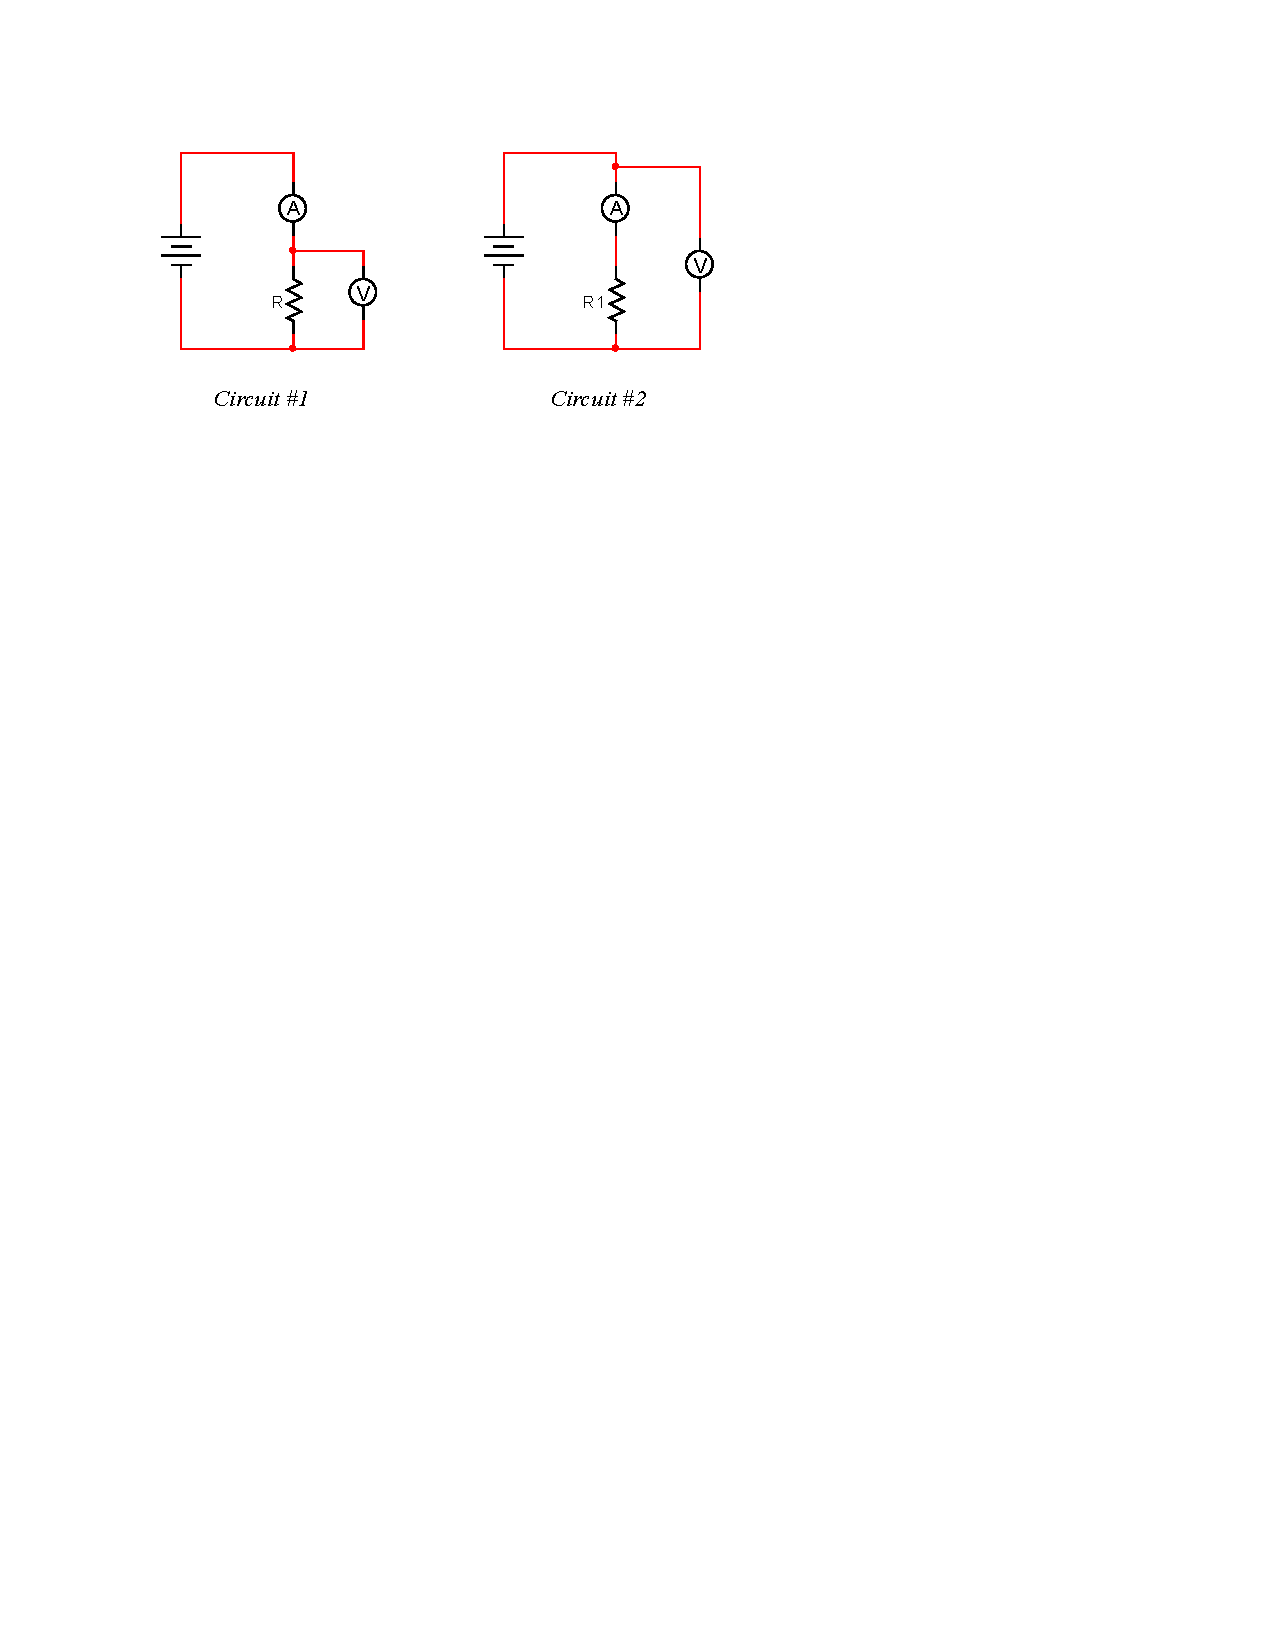
\includegraphics{M_problems/the_basics/I_V_measurements.pdf}
\index{color page}
\end{center}
\end{Exercise}
\begin{Answer}
(a) circuit \#1 (c) circuit \#2 (d) too high (e) circuit \#1
\end{Answer}

%\newcommand{\figuretoright}{3} {%
	%#1 is the picture width
	%#2 is the text to the right


%--------------------------------------------------------------------------------------------------------------
\begin{minipage}[t]{0.7\textwidth}
\begin{Exercise}
As shown in the figure to the right, two resistors in series may be thought of as a \textit{voltage divider}, 
where the output voltage $V_{\rm out}$ is a fixed fraction of the input voltage $V_{\rm in}$.  
Derive a general expression for $V_{\rm out}$ in terms of $R_1$, $R_2$, and $V_{\rm in}$.  Note that the word \textit{derive} means to
demonstrate using some mixture of mathematical statements along with some words and possibly a picture.
\end{Exercise}
\begin{Answer}
$\displaystyle V_{\rm out} = V_{\rm in}\left(\frac{R_2}{R_1+R_2}\right)$.  (Hint: start by finding the current through the resistors.)
\end{Answer}
\end{minipage}
\begin{minipage}[t]{0.3\textwidth - 4pt}

\smallskip
\hfill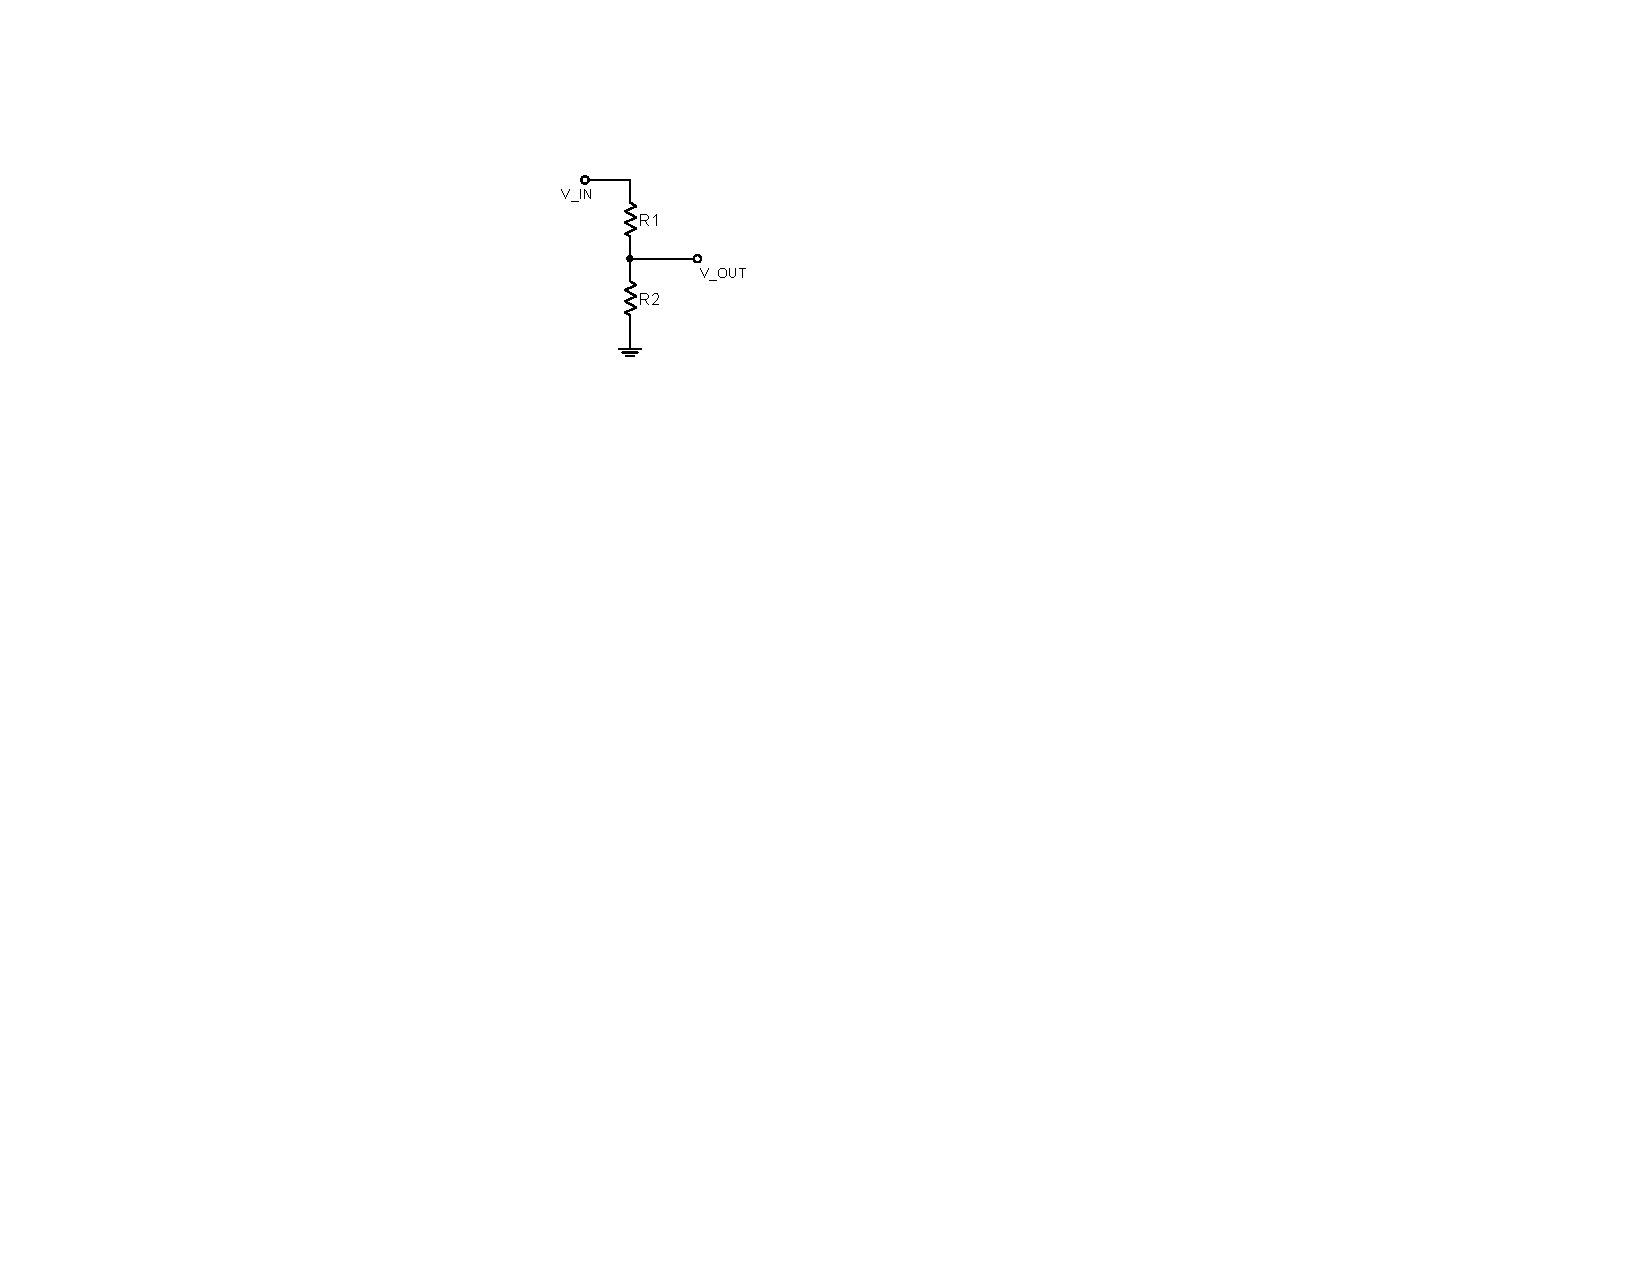
\includegraphics{M_problems/the_basics/voltage_divider.pdf}
\end{minipage}

%--------------------------------------------------------------------------------------------------------------
\begin{Exercise}
\label{prob_impedance_matching}
Consider a power supply like the battery depicted in problem MA2, in which the supply has an internal voltage $\varepsilon$ and an internal resistance $R_{\rm int}$, and where the supply will be connected to a load resistance $R_{\rm load}$.  (Feel free to call the resistances ``$R_1$'' and ``$R_2$'' if you prefer.)
(a)~Write an expression for the power $P_{load}$ dissipated in the load resistor, 
in terms of only $\varepsilon$, $R_{\rm int}$, and $R_{\rm load}$.  
(b)~Suppose that the internal resistance $R_{\rm int}$ of the source is fixed, and you cannot change it.  Derive an expression for the optimal value you should choose for $R_{\rm load}$ in order to \textit{maximize} the power dissipated in the load.
(c)~Now suppose instead that it is the load resistance $R_{\rm load}$ that is fixed and unchangeable.  Derive an expression for the optimal value you should choose for $R_{\rm int}$ in order to \textit{maximize} the power dissipated in the load.
(d)~Based on your answer to part (c), it turns out that some battery types are just better at delivering high load power than others.  Do a little Googling to find how the internal resistance of lithium ion batteries compares to, say, alkaline batteries.  Are there any other battery types that stand out as particularly good or particularly bad?
\end{Exercise}
\begin{Answer}
(b) $R_{\rm load} = R_{\rm int}$ (c) The correct answer is NOT $R_{\rm int} = R_{\rm load}$.
\end{Answer}

%--------------------------------------------------------------------------------------------------------------
\begin{Exercise}
You may have wondered why resistors have the odd values that they often do: for instance, why $2.2\kohm$ and $4.7\kohm$ instead of $2\kohm$ and $5\kohm$? To find out why, check out the Wikipedia entry entitled ``E series of preferred numbers.'' 
\begin{enumerate}[label=(\alph*),nosep]
\item Which set of numbers do the resistors in your kit follow?  (E3? E6? E192?) 
\item In a single sentence of your own words, how are the numbers in that specific sequence calculated?
\end{enumerate}
With the resistors that you have, it is almost always possible to combine just two of them either in series or in parallel to generate virtually any equivalent resistance you want to an accuracy of better than 1\%.  There are various handy online calculators to help you do so, such as the one at \url{https://svajkaj.com/}.  Use this online calculator (or a different one, I guess) to calculate the following:
\begin{enumerate}[resume*]
\item What is the best way to approximate $7.0\kohm$ using just two E6 resistors?
\item What is the best way to approximate $2.7\kohm$ using just two E6 resistors?
\end{enumerate}
\end{Exercise}

%--------------------------------------------------------------------------------------------------------------
\begin{Exercise}
A student has connected the circuit below to their 5~V power supply, expecting a voltmeter reading of $V=2.5$~volts.  Which of the causes listed on the right could lead to each of the symptoms on the left?  More than one answer may apply.

\begin{minipage}[t]{0.35\textwidth}
\textbf{Symptoms}
\begin{enumerate}[nosep,wide]
\item The voltmeter reads 2.58 volts. % i,  within tolerances
\item The voltmeter reads 2.76 volts. % c,  current meter on microvolts
\item The voltmeter reads 4.98 volts. % a,d,e,g  not grounded, or R2 shorted to 5V, or R1 leads touching, or blown fuse. 
\item The voltmeter reads 1.62 volts.  % h, R1 is 10k
\item The voltmeter reads about 0 volts.       % b, R2 shorted 
\end{enumerate}
\end{minipage}%
\begin{minipage}[t]{0.42\textwidth}
\textbf{Causes}
\begin{enumerate}[label=(\alph*),nosep,labelindent=0in]
\item The two leads of $R_1$ are touching each other (``shorted'')
\item The two leads of $R_2$ are touching each other (``shorted'')
\item The current meter is on the $\mu$A scale. 
\item $R_2$ has not been connected to ground.
\item The current meter has a blown fuse.
\item The voltmeter has a blown fuse.
\item One side of $R_2$ has been connected to the 5~V supply.
\item $R_1$ is actually a $10\kohm$ resistor.
\item The circuit is built correctly and the output is within the range expected for the tolerances of the components.
\end{enumerate}
\end{minipage}%
\begin{minipage}[t]{0.22\textwidth}
%Testing testing

\phantom{need text here}

\vspace*{-0.3in}

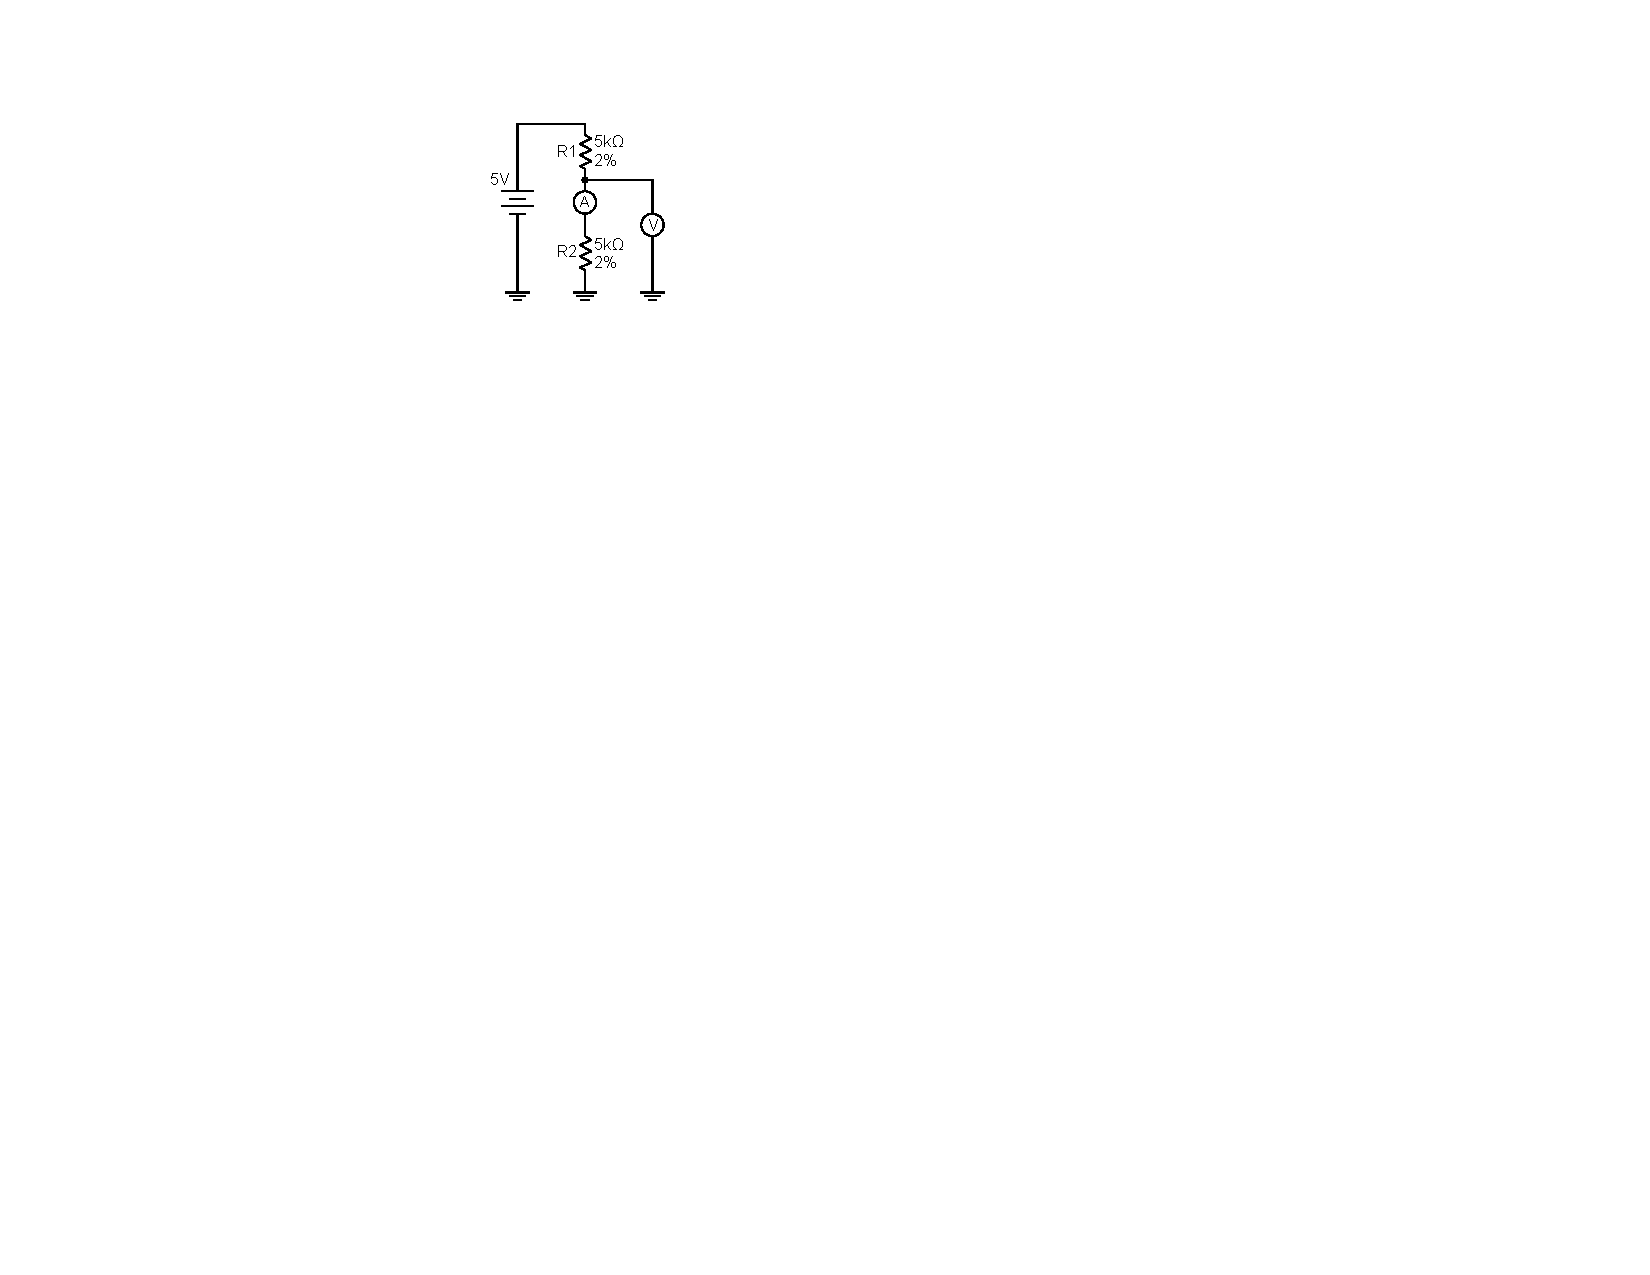
\includegraphics{M_problems/the_basics/troubleshooting_IV_series.pdf}

\end{minipage}%
\end{Exercise}
\begin{Answer}
Of the nine lettered causes (a) thru (i), all but one gets used, and none are used more than once.  Feel free to check your answers for each symptom 1 thru 5 with me; I will tell you what's wrong and let you try again.
\end{Answer}


%--------------------------------------------------------------------------------------------------------------
\begin{Exercise}
A student has constructed the circuit to the right, expecting an adjustable output voltage $V_{\rm out}$ in the range of 2~V to 4~V.  Which of the causes on the right \textit{could} lead to each of the symptoms on the left?  More than one answer may apply.

\begin{minipage}[t]{0.30\textwidth}
\textbf{Symptoms}
\begin{enumerate}[nosep,wide]
\item  $V_{\rm out}$ range is 2~V to 4~V. % g, within tolerances
\item  $V_{\rm out}$ is a constant 6~V.     % a, not grounded
\item  $V_{\rm out}$ is a constant 4~V.     % d, V_out connected to pin 1
\item  $V_{\rm out}$ range is 3~V to 6~V. % b, Two leads of R1 are touching.
\item  $V_{\rm out}$ range is 2~V to 3~V. % e, pins 2 and 3 shorted together.
\item  $V_{\rm out}$ range is 1~V to 2~V. % f, Input voltage is 3 V
\end{enumerate}
\end{minipage}
\begin{minipage}[t]{0.54\textwidth}
\textbf{Causes}
\begin{enumerate}[label=(\alph*),nosep,labelindent=0in]
\item $R_2$ has not been connected to ground. %
\item The two leads of $R_1$ are touching each other.
\item The two leads of $R_2$ are touching each other.
\item $V_{\rm out}$ connected to pin 1, not pin 2.
\item Pins 2 and 3 are connected (``shorted'') together.
\item $V_{\rm in}$ connected to 3 volts.
\item The circuit is correct and the output is within the range expected for the tolerances of the components.
\end{enumerate}
\end{minipage}
\begin{minipage}[t]{0.15\textwidth}

%Testing testing
\phantom{need text here}

\vspace*{-0.3in}

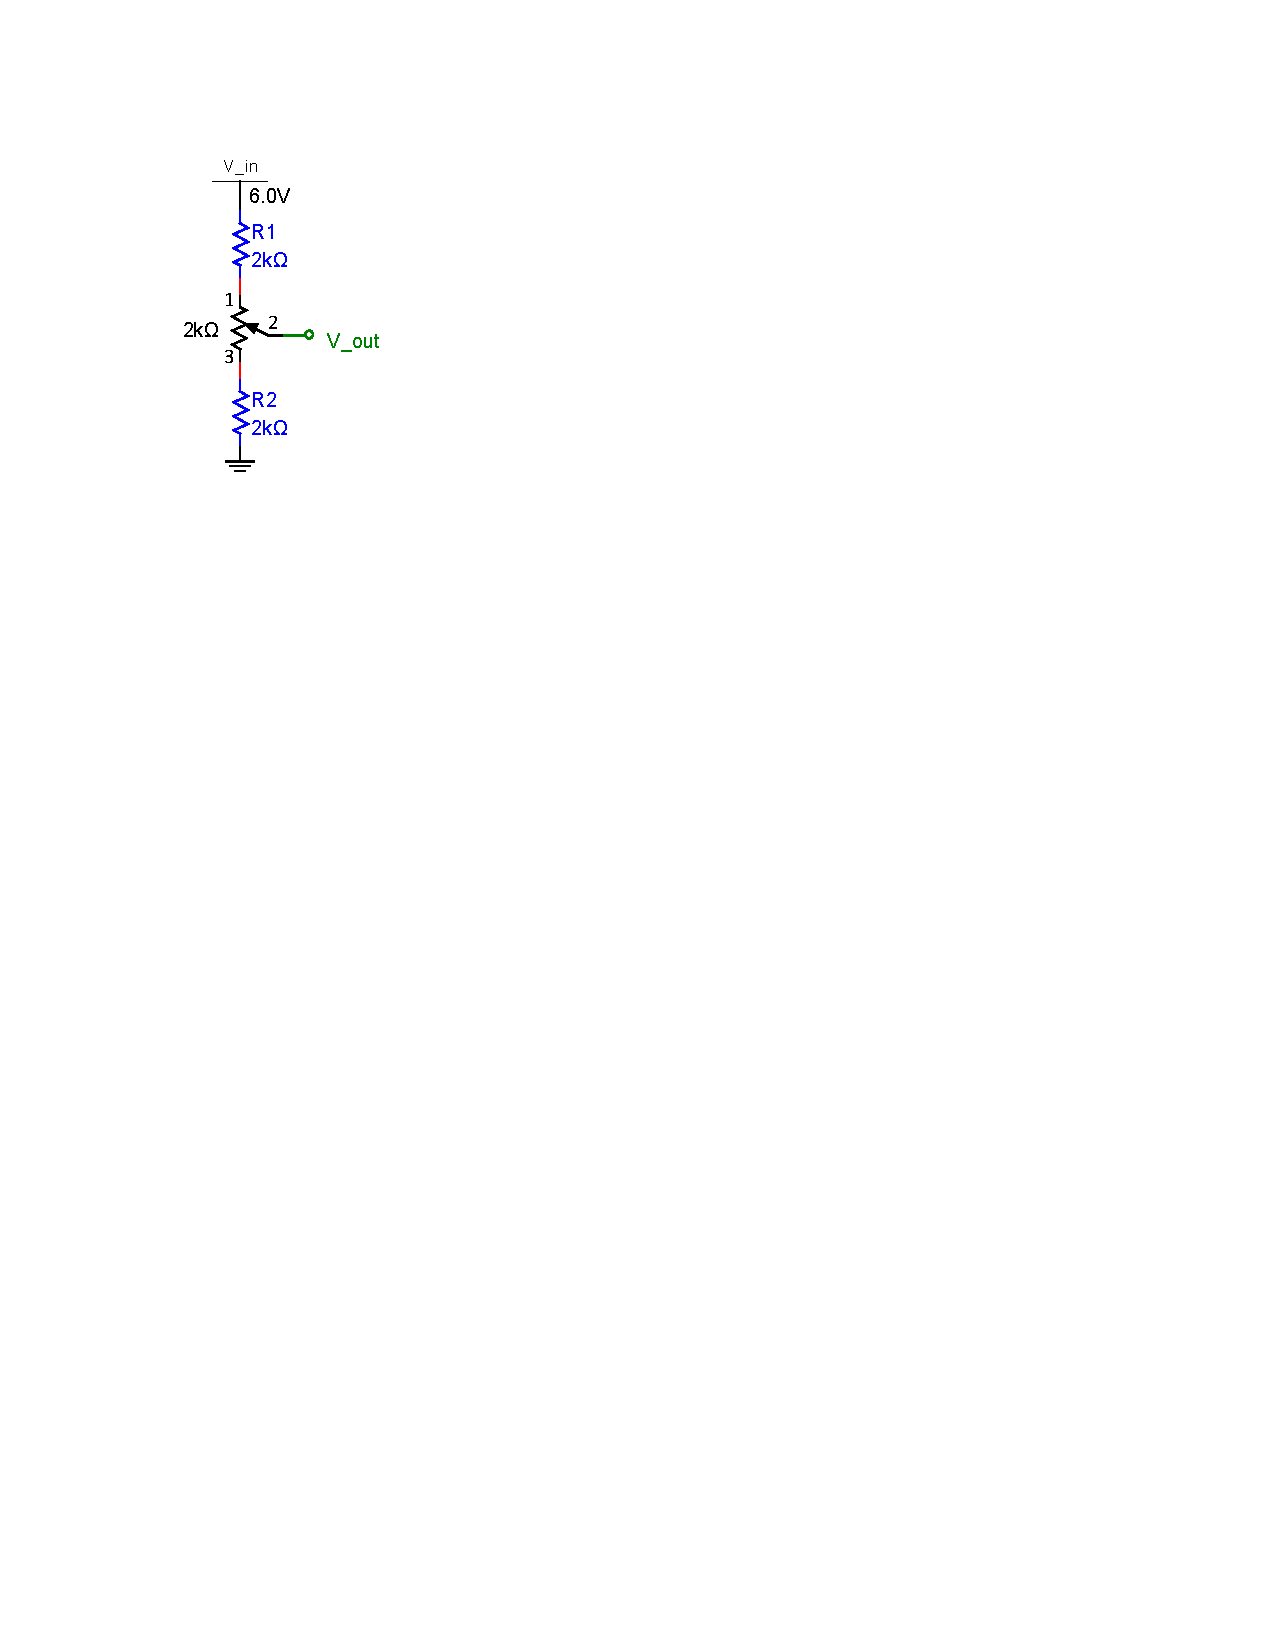
\includegraphics[scale=0.65]{M_problems/the_basics/troubleshooting_voltage_divider_masked.pdf}

\end{minipage}%
\end{Exercise}
\begin{Answer}
Each symptom 1 through 6 has exactly one cause from the list.  Feel free to check your answers for each symptom with me; I will tell you what's wrong and let you try again.
\end{Answer}

%--------------------------------------------------------------------------------------------------------------
\begin{Exercise}
(a)~Design a voltage divider that will guarantee that $V_{\rm out}/V_{\rm in}=0.500$ using a trimpot and two fixed resistors: a $15\kohm$ and $15\kohm$ both 2\% tolerance.  (b)~Design a voltage divider that will guarantee that $V_{\rm out}/V_{\rm in}=1/3$ using a trimpot and two fixed resistors: a $100\kohm$ and $200\kohm$ both 1\% tolerance.  For both parts, use the minimum value of trimpot that will guarantee the correct output.  (Note that ``Design'' means to draw the circuit diagram showing the values of all components.)
\end{Exercise}
\begin{Answer}
(a) $600\ohm$ (b) $4\kohm$
\end{Answer}

%--------------------------------------------------------------------------------------------------------------
\begin{Exercise}
%In this problem, you will examine contact resistance in a trimpot and how to minimize its effects.
A common problem with trimpots and other potentiometers is that the movable wiper (pin 2 in the drawing below) doesn't always make good electrical contact with the resistive material between pins 1 and 3.  The resulting \textit{contact resistance} is particularly pernicious because it can fluctuate wildly over time or when the trimpot is adjusted, leading to effects that are both undesirable and unpredictable.

%pic of contact resistance
\begin{center}
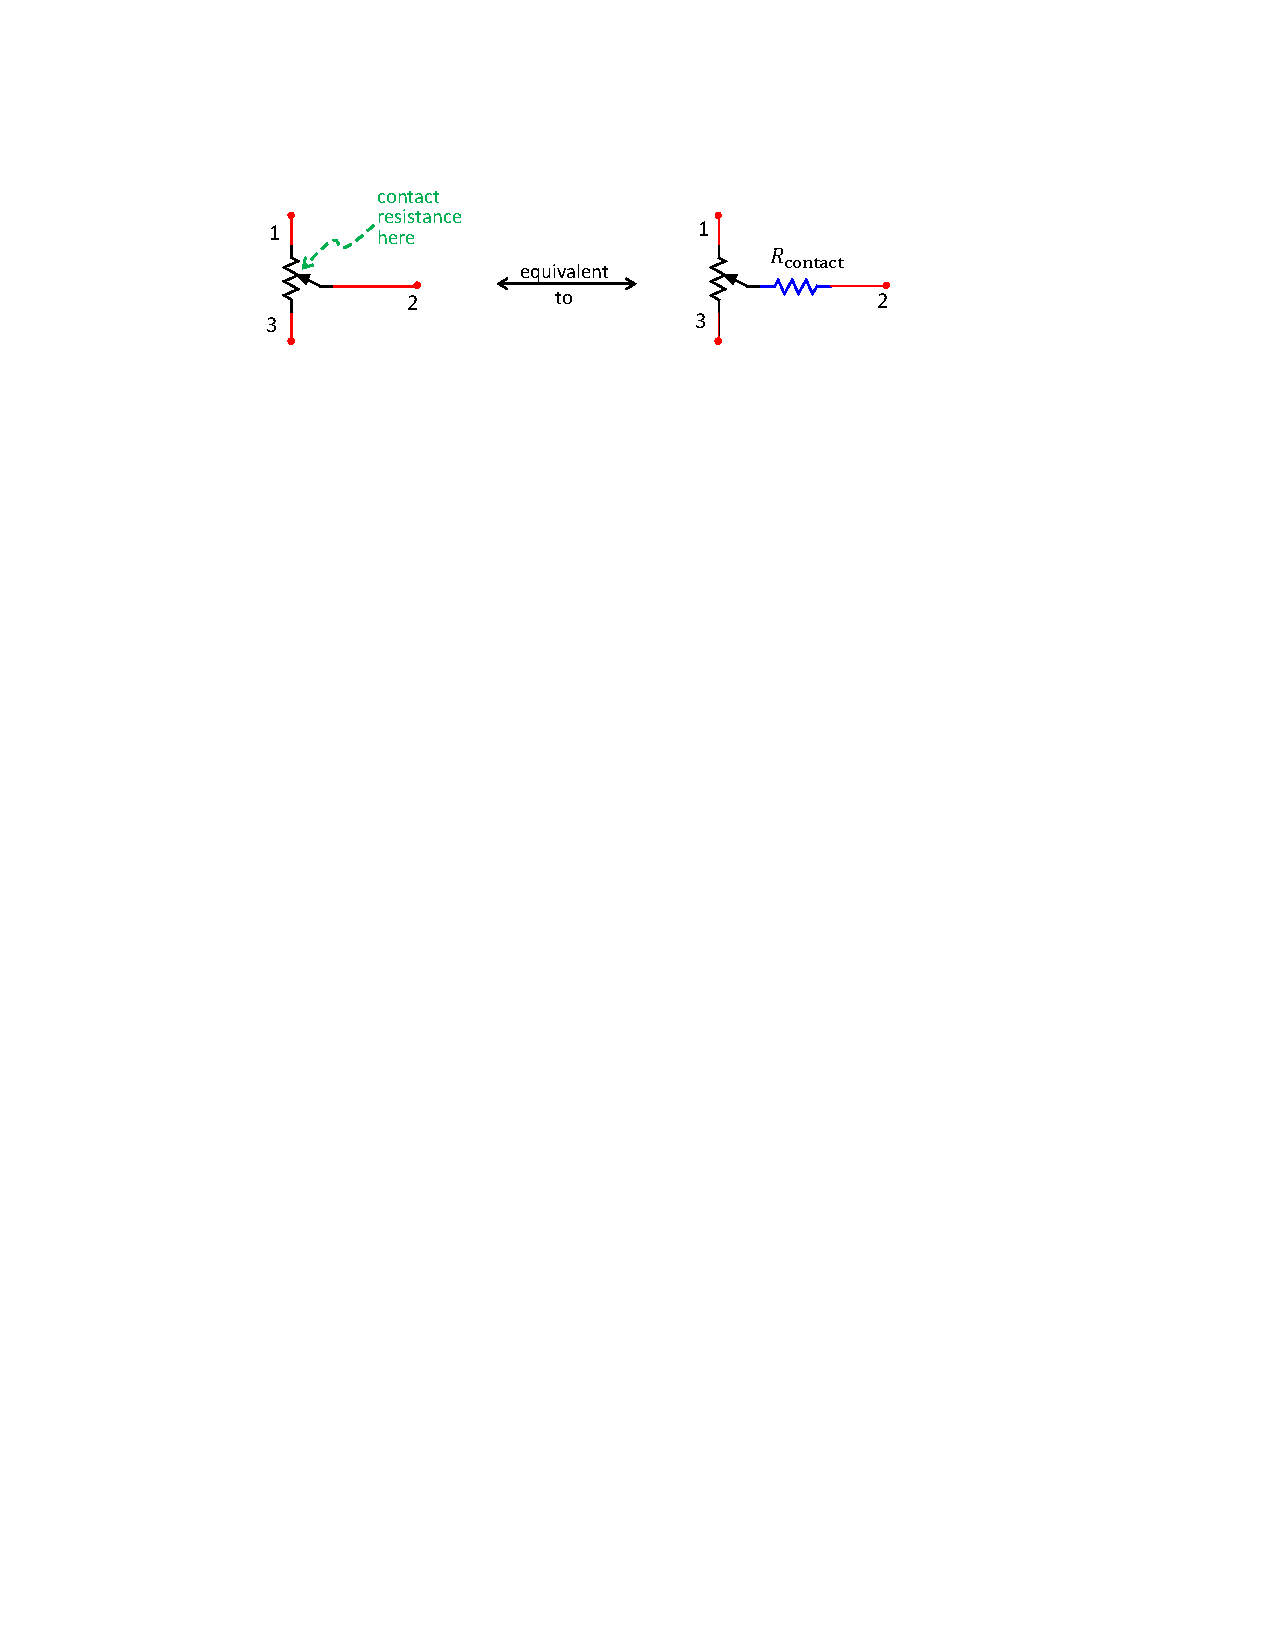
\includegraphics[scale=0.80]{M_problems/the_basics/contact_resistance_defined.pdf}
\end{center}

In the drawing below, the standard way to make a voltage divider is shown in Design~1, on the left.  
\begin{enumerate}[label=(\alph*),nosep]
\item What is the ideal output voltage range for Design~1, assuming that the output is connected to an infinitely large impedance ($R_{\rm load}=\infty$)? (in practice, the output of a voltage divider is almost always connected to something with a high input impedance---think of your voltmeter with $R_{\rm load}=10\Mohm$, for instance.)
\item What is the actual output range for Design~1 if the output is connected to a load with  $R_{\rm load}=1\Mohm$?  
\item How does the actual output range in (b) change with an additional contact resistance $R_{\rm contact}=1\kohm$?  
\end{enumerate}

%pic of three voltage divider circuits
\begin{center}
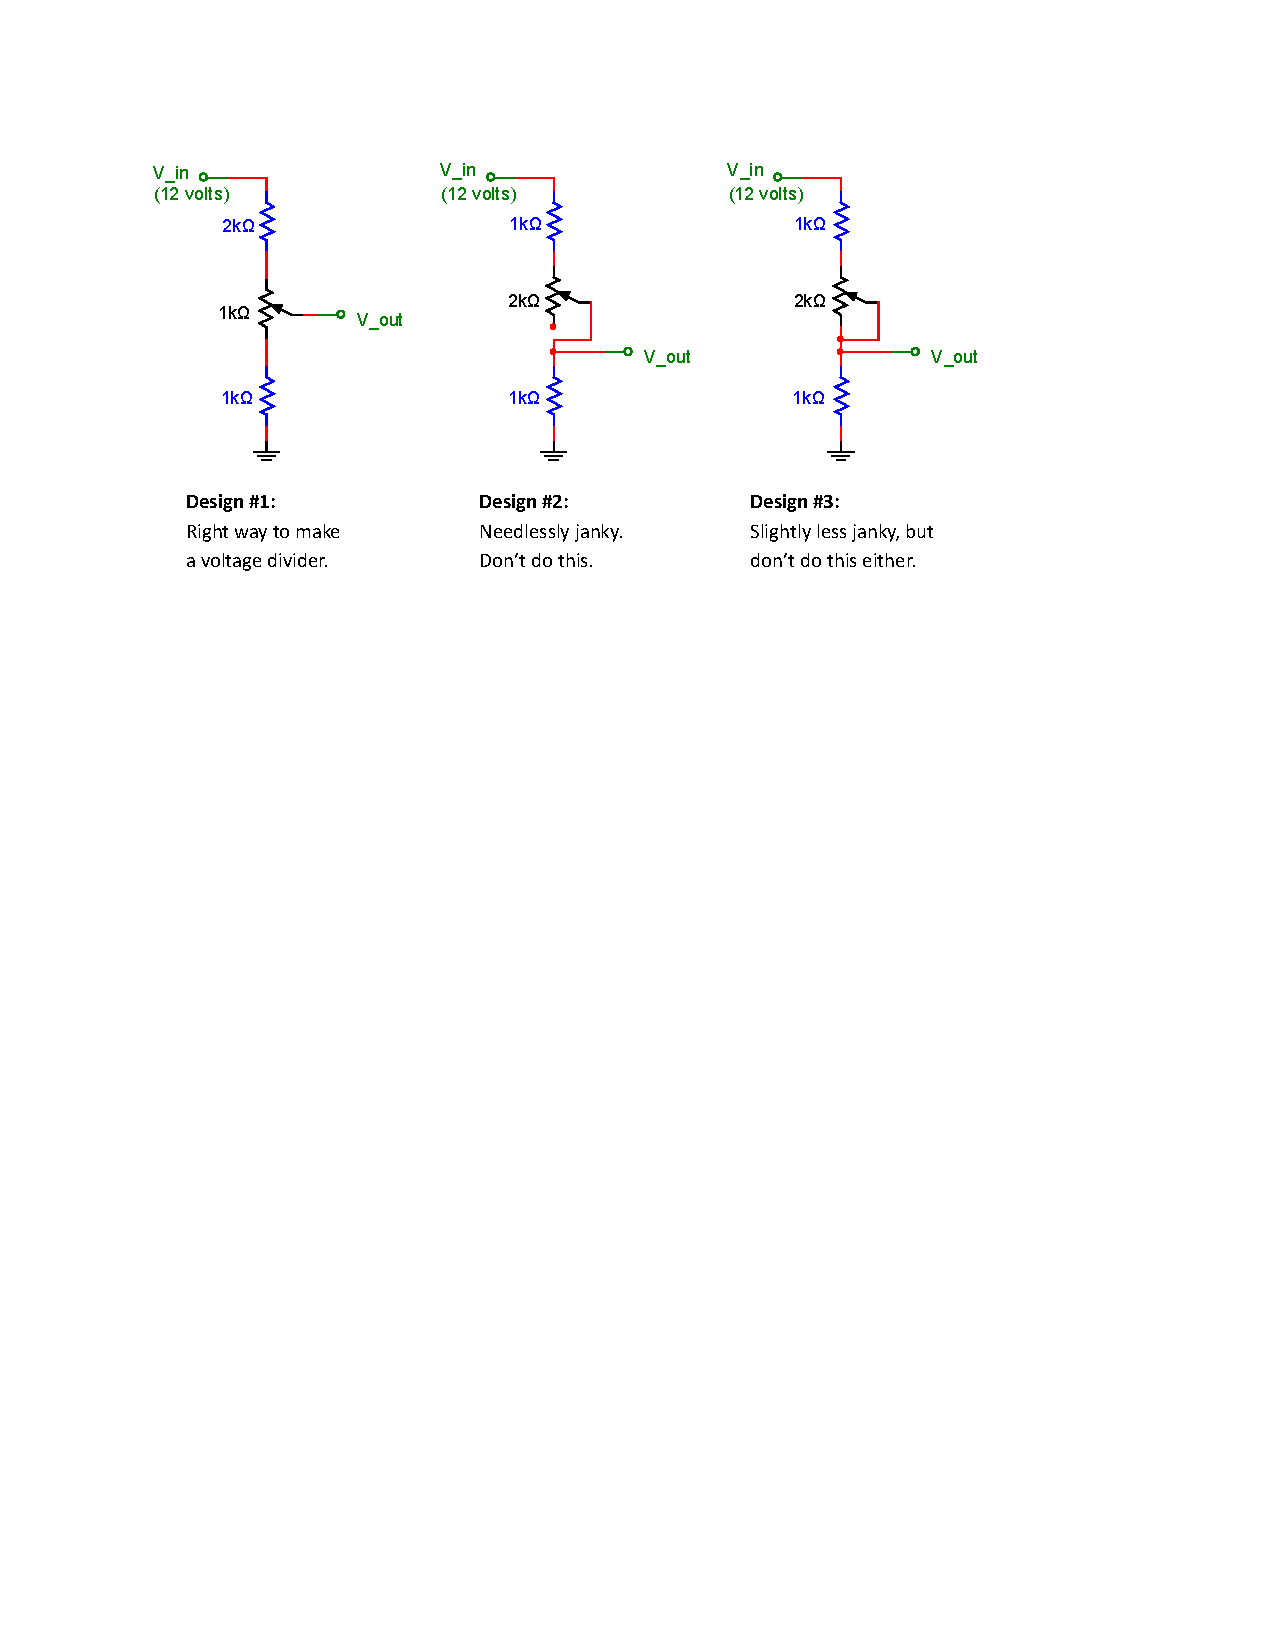
\includegraphics[scale=0.80]{M_problems/the_basics/voltage_divider_contact_resistance.pdf}
\end{center}

Your answers for parts (b) and (c) demonstrate that Design~1 is not affected much by contact resistance.
Designs~2 and~3 above are also ways to build a voltage divider, but
you'll see now that these are much more sensitive to changes in contact resistance.

\begin{enumerate}[resume*]
\item Convince yourself that with with $R_{\rm contact}=0$, Designs~2 and~3 give the same output range as Design~1.  You can assume here and for the remaining parts of this problem that $R_{\rm load}=\infty$.
\item What is the output range for Design~2 with $R_{\rm contact}=1\kohm$? What about with $R_{\rm contact}=\infty$?
\item What is the output range for Design~3 with $R_{\rm contact}=1\kohm$? What about with $R_{\rm contact}=\infty$?
\item Why is Design~3 better than Design~2?
\end{enumerate}
In general, you want as little current as possible to flow through the wiper of a potentiometer, to minimize the effect of contact resistance.  You very rarely need to use a potentiometer as a two-terminal variable resistor, but if you do you should always connect the wiper lead to one of the outer leads as in Design 3.
\end{Exercise}
\begin{Answer}
(a)~3.0 to 6.0~volts.  \\
(b)~$2.997\,751\,686$ to $5.994\,005\,994$~volts. ($R_{\rm load}$ changes the output voltages by about 0.1\%.)\\
(c)~$2.997\,753\,931$ to $5.994\,011\,976$~volts. ($R_{\rm contact}$ changes the output voltages by about 0.0001\%.)\\
(e)~2.4 to 4.0~volts for $R_{\rm contact} =1\kohm$, or constant 0~V for $R_{\rm contact} =\infty$.\\
(f)~3.0 to 4.5~volts for $R_{\rm contact} =1\kohm$, or constant 3~V for $R_{\rm contact} =\infty$.\\
(g)~With contact resistance, output of Design 3 is always closer to intended range than Design 2.  In fact, the output of Design 3 will never be \textit{outside} of the intended range, though the full intended range may not be accessible.
\end{Answer}

%--------------------------------------------------------------------------------------------------------------
\begin{Exercise}
A sinusoidal voltage with an amplitude of 10~V and a frequency of 0.25~Hz is placed across a load resistance of $220\ohm$.  (a)~What is the maximum \textit{instantaneous} power dissipated in the resistor?  (b) What is the \textit{average} power dissipated in the resistor?
\end{Exercise}
\begin{Answer}
(a) 0.45 W (b) 0.23 W
\end{Answer}

%--------------------------------------------------------------------------------------------------------------
\begin{Exercise}
The periodic waveform shown below is 20~V for $10~\mu$s and $-5$~V for $15~\mu$s.
\begin{center}
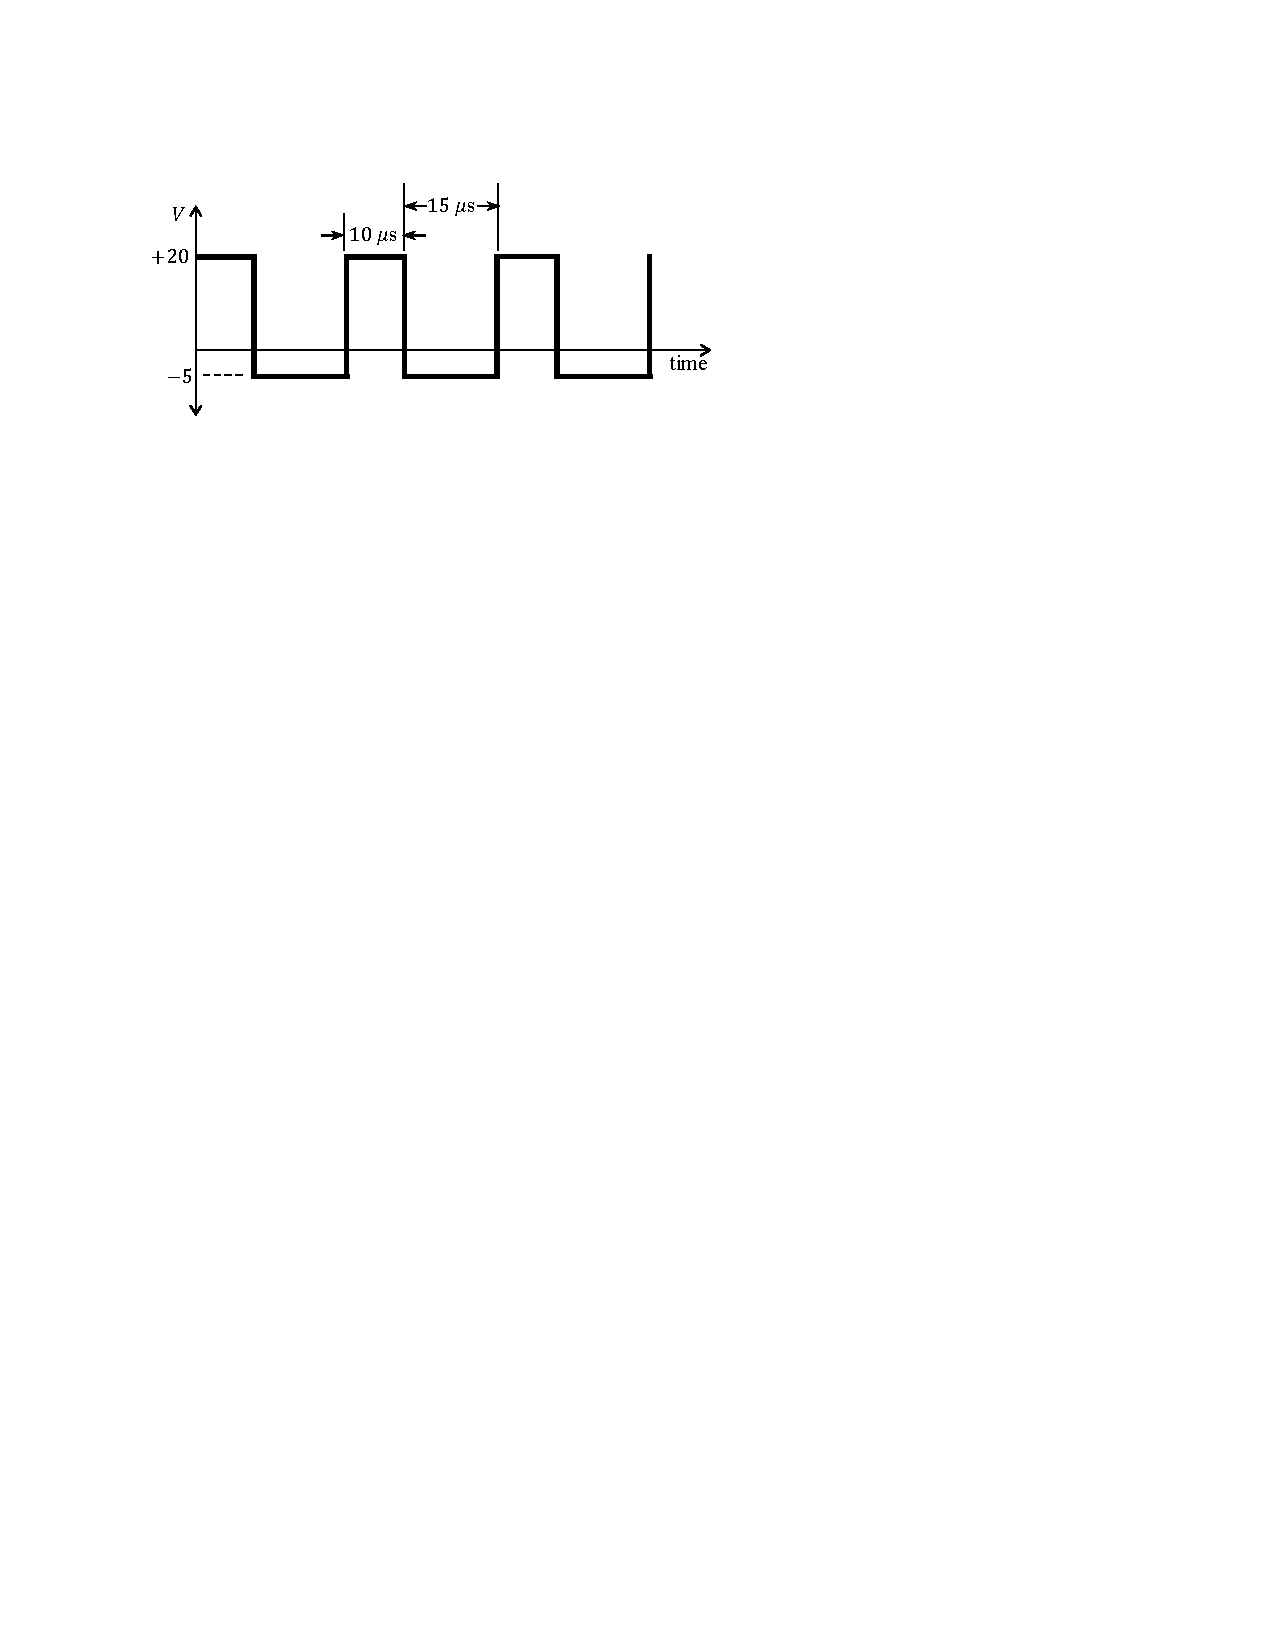
\includegraphics{M_problems/the_basics/irregular_periodic_wave.pdf}
\end{center}

\begin{enumerate}[label=(\alph*),nosep]
\item What range of voltages is displayed on an oscilloscope if the signal is measured using DC coupling?
\item What range of voltages is displayed on an oscilloscope if the signal is measured using AC coupling?
\item What is the RMS value of this signal as measured using DC coupling?
\item What is the RMS value of this signal as measured using AC coupling?
\end{enumerate}
\end{Exercise}
\begin{Answer}
(b)$-10$ to 15 V (c)~13.23~V (d)~12.25~V 
\end{Answer}

%--------------------------------------------------------------------------------------------------------------
\begin{Exercise}
(a)~Find the RMS voltage of a periodic sawtooth wave which rises linearly from 0 to $V_{\rm max}$ and falls instantaneously to zero, such that $V=V_{\rm max}t/\tau$, where $\tau$ is the period.  Yes, you will need to compute an integral to answer this question. 
(b)~Use your result from part (a) to find the RMS voltage of a triangle wave (as from your function generator) that oscillates between $-V_{\rm peak}$ and $+V_{\rm peak}$.
\end{Exercise}
\begin{Answer}
(a) $0.58V_{\rm max}$
\end{Answer}

%Ideas for additional problems:
%uncertainty, like 132 problem?
%pictures of breadboards with resistors, where students draw circuit diagram or say if resistors are in parallel or series

%\vfill
%\pagebreak[3]

\vspace{0.7in}

\textbf{Answers to Selected {\thesubsection} Problems:}
\label{the_basics_prob_answers}
%\shipoutExercise
\shipoutAnswer

\cleardoublepage

\subsection{Two Important Kinds of ICs} 

%\DTMnewdatestyle{dateupdated}{〈definition 〉

Answers to M\Alph{subsection} problems are on page \pageref{opamps_digital_prob_answers}.  \textbf{\textcolor{red}{Updated \DTMnow.}}

%--------------------------------------------------------------------------------------------------------------
\begin{Exercise}
\label{prob_calculate_inverting_amp_gain}
For the circuit shown below, suppose that $V_{\rm in} =3$~volts.  
Find (a)~$V_+$ and $V_-$, 
(b)~$I_{R3}$ and $I_{R4}$, 
(c)~$\Delta V_{R3}$ and $\Delta V_{R4}$.  
(d)~What direction does current flow in $R_3$ and in $R_4$: to the left or to the right? 
(e)~Which direction does current flow through the op-amp's output? 
(f)~What is $V_{\rm out}$?

\vspace{-0.15in}
\begin{center}
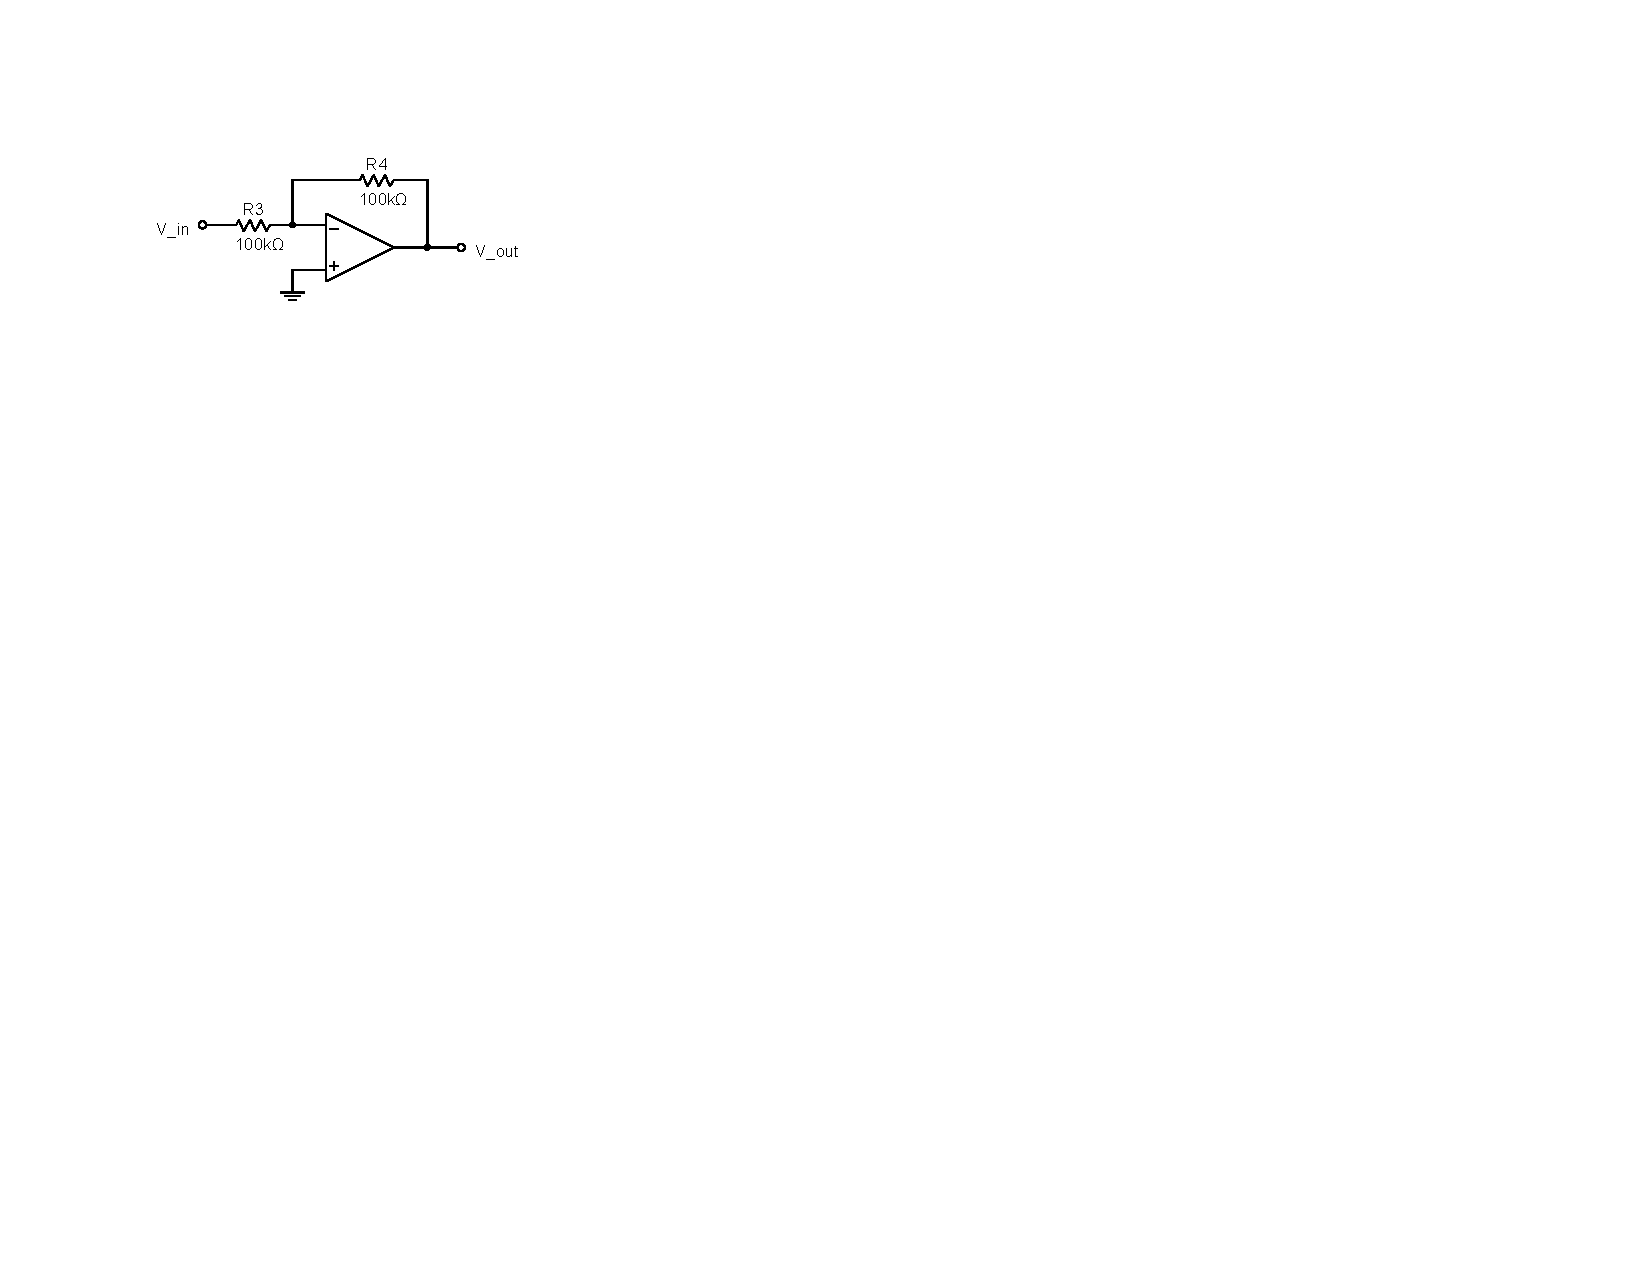
\includegraphics{M_problems/opamps_digital/inverting.pdf}
\end{center}
\vspace*{-0.25in}
\end{Exercise}
\begin{Answer}
(a) 0 (b) $30~\mu$A (c) 3 volts (d) both flow left to right (e) right to left (f) $-3$ volts
\end{Answer}

%--------------------------------------------------------------------------------------------------------------
\begin{Exercise}
\label{prob_thevenin_equiv_for_2V_supply}
A student named Ralph has used a voltage divider to build a 2-volt DC voltage supply, shown below on the left.  It turns out there is a very useful theorem by a fellow named Thevenin, which says roughly the following:
\begin{quote}
``Any collection of voltage sources and resistors (even the crazy middle figure below!) is functionally equivalent to a single voltage source $V_{\rm Th}$ and a single internal resistance $R_{\rm Th}$ as shown on the right.  No measurement at $V_{\rm out}$ can distinguish between the two circuits.''  ---L\'eon Charles Th\'evenin (heavily paraphrased).
\end{quote}
In this problem, you will calculate the values of $V_{\rm Th}$ and $R_{\rm Th}$ for the equivalent circuit of Ralph's voltage supply. 

\vspace{-0.15in}
\begin{center}
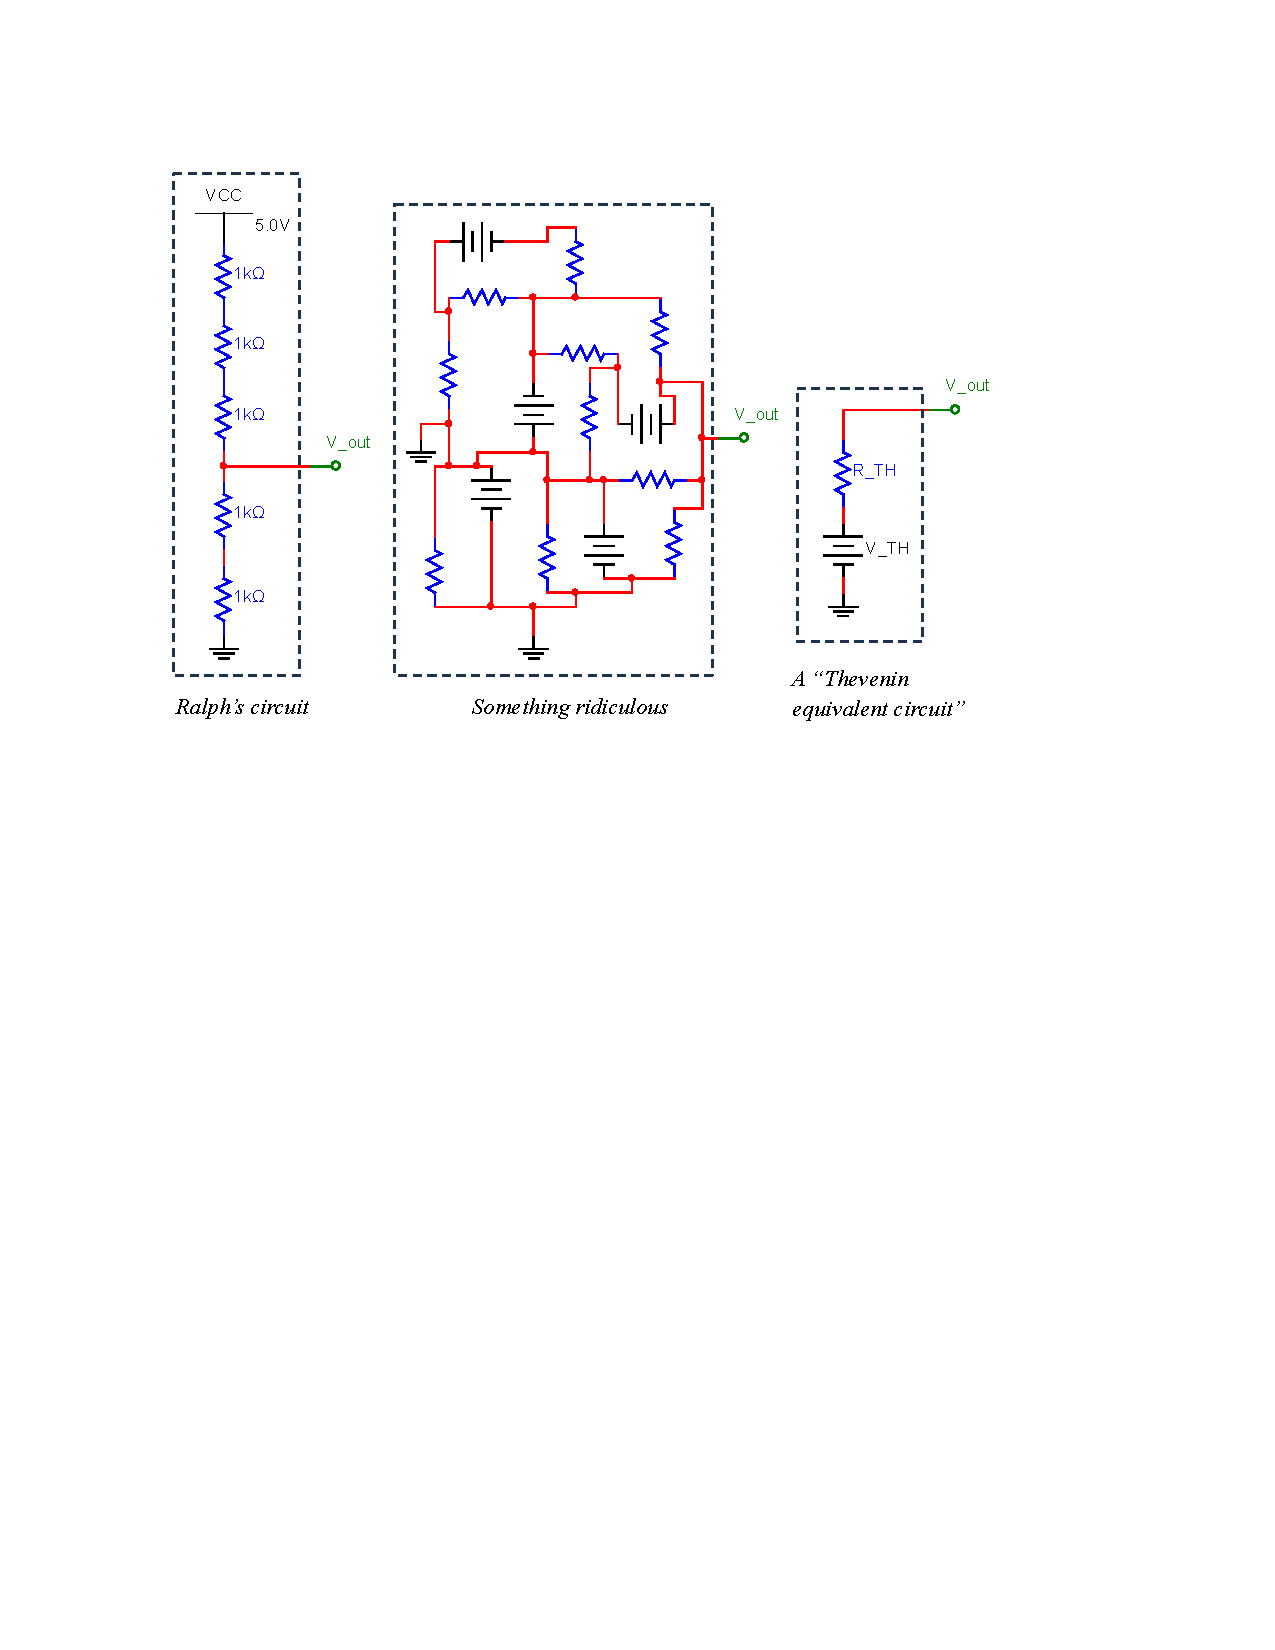
\includegraphics[scale=0.86]{M_problems/opamps_digital/thevenin_equivalence.pdf}
\index{color page}
\end{center}
\vspace{-0.25in}

\begin{enumerate}[label=(\alph*),nosep]
\item What is the open-circuit voltage of the Thevenin equivalent circuit on the right, in terms of $V_{\rm Th}$ and $R_{\rm Th}$? 
\item What is the short-circuit current of the Thevenin equivalent circuit on the right? 
\item What is the open-circuit voltage of Ralph's circuit?  
\item What is the short-circuit current of Ralph's circuit?  
\item From your previous parts what are the values of $V_{\rm Th}$ and $R_{\rm Th}$ for Ralph's circuit?  
\item Ralph does the same calculation that you did, and says, ``Hey, it looks like the output impedance of my circuit is 1.2~k$\Omega$.''  Is \textit{output impedance} the right thing for Ralph to call it?
\end{enumerate}
For more help using Thevenin's theorem, see Appendix \ref{thevenin_equivalence}.
\end{Exercise}
\begin{Answer}
(a) It's just $V_{\rm Th}$ (b) $V_{\rm Th}$ and $R_{\rm Th}$ (c) 2 V (d) 1.67 mA (e) 2 V and 1.2 k$\Omega$ (f)~Sure, that's basically what it is.  In this context, ``output impedance/resistance'' or ``internal resistance'' or ``Thevenin equivalent resistance'' basically all mean the same thing.
\end{Answer}


%--------------------------------------------------------------------------------------------------------------
\begin{Exercise}
In this problem, you will test whether Ralph's circuit in the previous problem is equivalent to a Thevenin equivalent circuit with $V_{\rm Th}=2$~volts and $R_{\rm Th}=1.2\kohm$, by checking the behavior of a circuit with a single, arbitrarily chosen load resistor $R_{\rm L}$. Suppose a load  $R_{\rm L}=2.7\kohm$ is connected between Ralph's output and ground.  (a)~Calculate the voltage across and current through $R_{\rm L}$ by analyzing the circuit in the diagram below on the left.  (b)~Calculate the voltage and current for $R_{\rm L}$ by analyzing the circuit in the diagram below on the right.  (c)~Are they the same?  (d)~Does this count as a ``proof'' of Thevenin's theorem?
\begin{center}
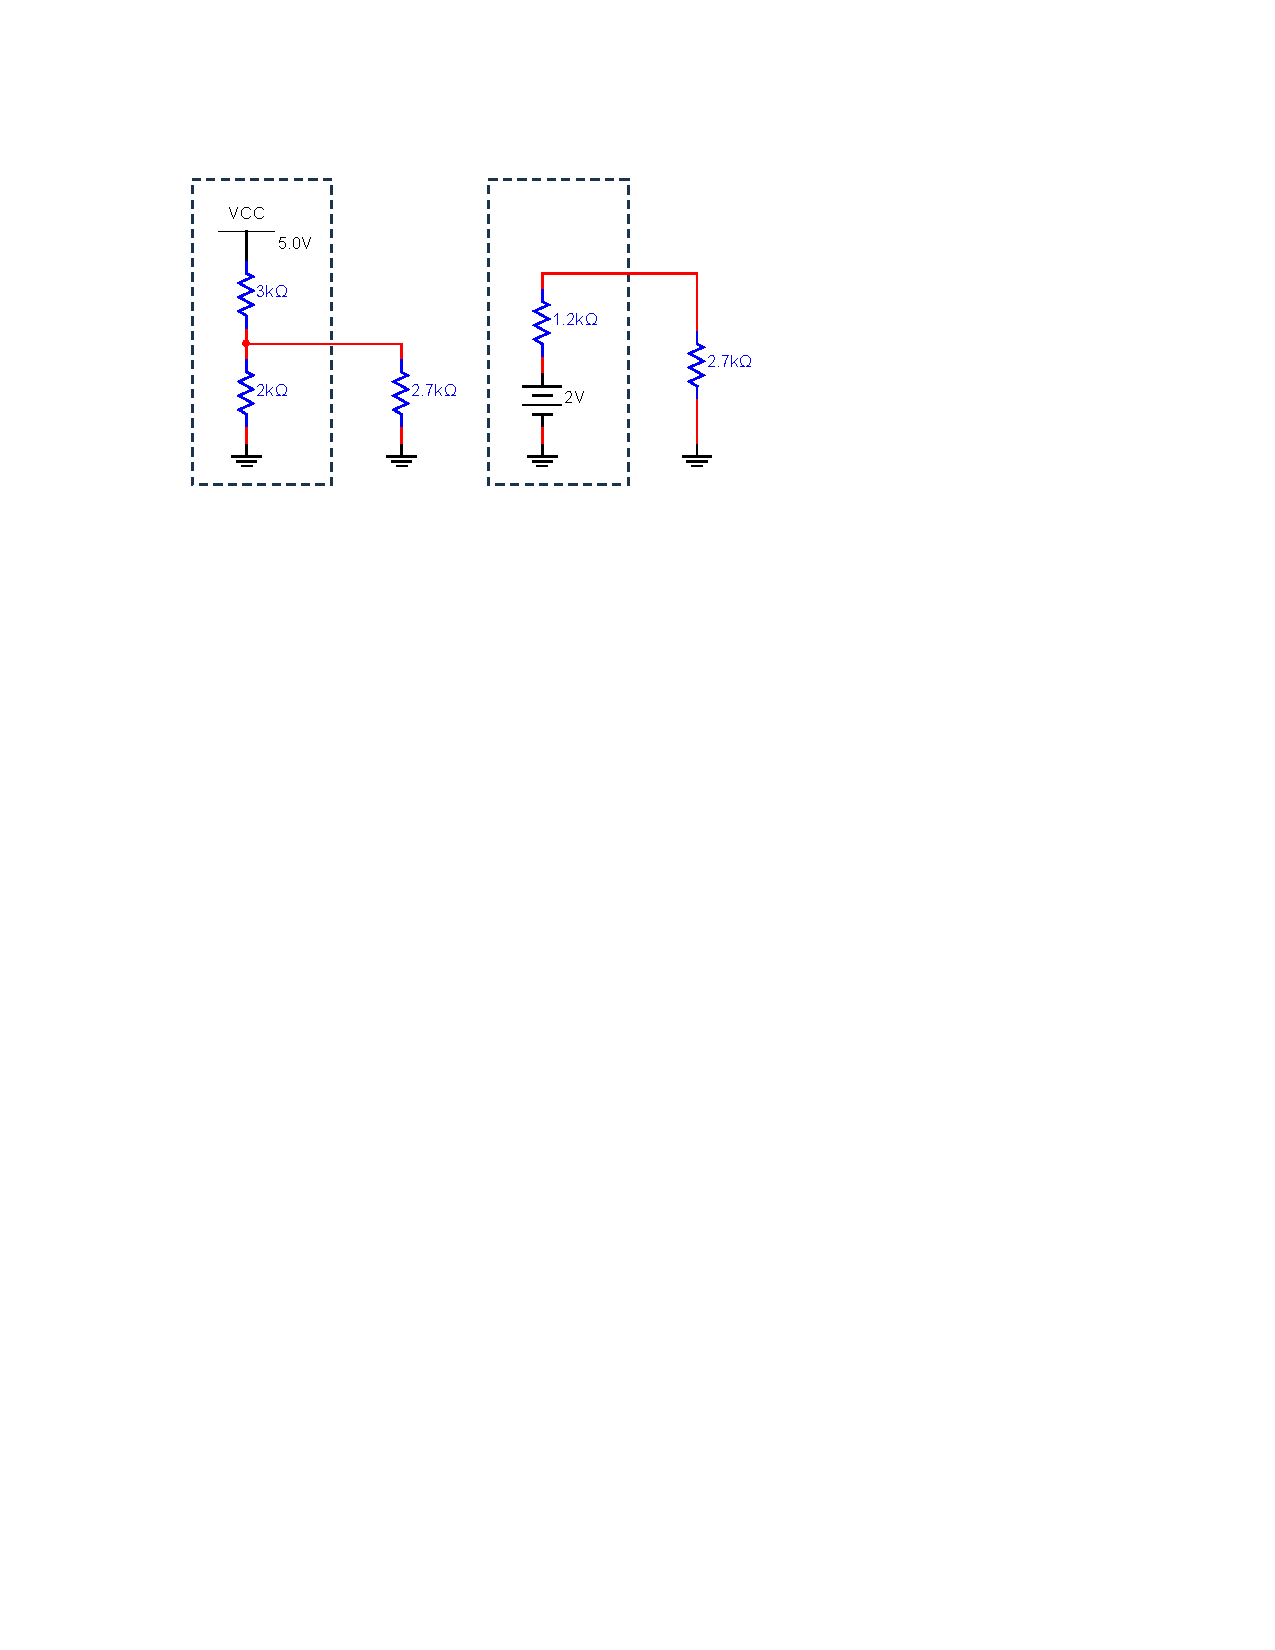
\includegraphics[scale=0.9]{M_problems/opamps_digital/thevenin_equivalence2.pdf}
\index{color page}
\end{center}
\end{Exercise}
\begin{Answer}
(a)~1.38~V and 513~$\mu$A  (c)~They'd better both be the same! (d)~No, it's not a general proof, because you demonstrated it only for one specific load (a single $2.7\kohm$ resistor) connected to one specific circuit made by some fake guy named Ralph.  But if you see this kind of thing enough times, it does start to seem convincing.  :-)
\end{Answer}


%--------------------------------------------------------------------------------------------------------------
\begin{Exercise}
\label{prob_amplifier_input_impedances}
(a) What is the input impedance of the inverting amplifier you built in Lab \ref{lab_op-amps}, part \ref{part_inverting_amplifier}?  
(b) By contrast, is the input impedance of the non-inverting amplifier you built in Lab \ref{lab_op-amps} part \ref{part_non-inverting_amplifier} larger or smaller than the inverting amplifier?
(c) What additional information would you need in order to calculate a numerical value for the input impedance of the non-inverting amplifier, and where would you go to find it?
\end{Exercise}
\begin{Answer}
(a) Hint: The input $V_+$ is at ground, and the op-amp adjusts its output to keep $V_- = V_+$.  This means that the $V_-$ input is essentially at 0 volts as well---what we call a \textit{pseudo ground}---and you can treat it as if the right side of resistor $R_3$ was simply connected directly to ground.
\end{Answer}

%--------------------------------------------------------------------------------------------------------------
\begin{Exercise}
Anna and Bob are building inverting amplifiers, just as you did in Lab \ref{lab_op-amps}, part \ref{part_inverting_amplifier}. Their goal is to use a 2-volt signal as an input to an inverting amplifier with a gain of $-1$.  Anna builds the circuit on the left (below), and Bob builds the circuit in the middle. 
(a)~Which of the two circuits works the way it's supposed to, and why does the other one \textit{not} work?
(b)~Carla is out of $100\kohm$ resistors, so she builds the circuit on the right.  Show how to calculate the output voltage of Carla's circuit \textit{specifically by using the results from problems
\textsl{\ref{prob_thevenin_equiv_for_2V_supply}} and
\textsl{\ref{prob_amplifier_input_impedances}}.}
\begin{center}
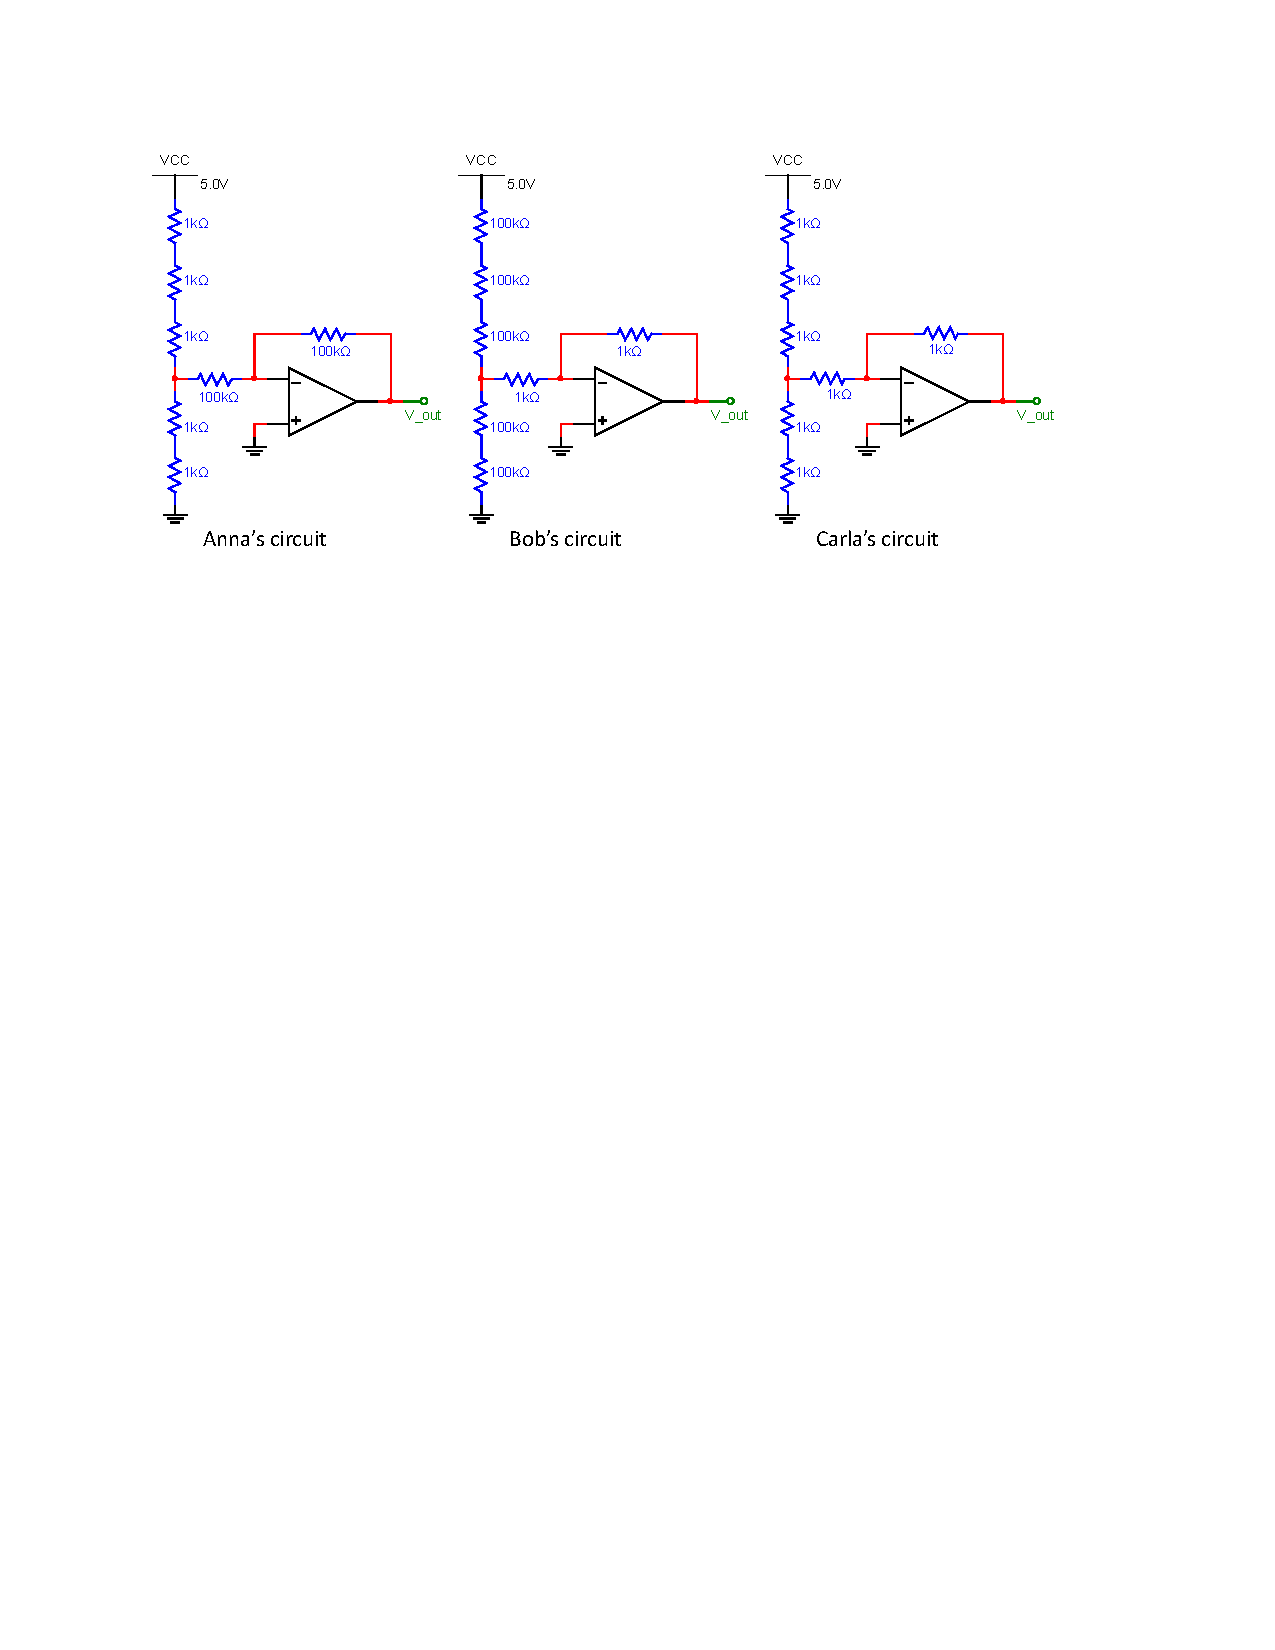
\includegraphics{M_problems/opamps_digital/anna_bob_carla.pdf}
\end{center}
\end{Exercise}
\begin{Answer}
(b) $-0.91$~volts
\end{Answer}


%--------------------------------------------------------------------------------------------------------------
\begin{Exercise}
Referring to the circuit diagrams in parts 
\ref{part_non-inverting_amplifier} and 
\ref{part_inverting_amplifier} of 
Lab \ref{lab_op-amps}, 
\textit{derive} (using a judicious mix of math, words, and/or pictures)  expressions for (a)~the gain $G$ of a non-inverting amplifier in terms of $R_1$ and $R_2$, and (b)~the gain $G$ of an inverting amplifier in terms of $R_3$ and $R_4$.
\end{Exercise}
\begin{Answer}
(a) $G=\left(R_1 + R_2\right) / {R_2}$ (b) $G={-R_4}/{R_3}$.  General hint: In problem \ref{prob_calculate_inverting_amp_gain} you worked out the gain of an inverting amplifier with specific resistor values, and you can follow the same kind of logic here.
\end{Answer}


%--------------------------------------------------------------------------------------------------------------
\begin{Exercise}
A source with an output impedance of 50 ohms produces an open-circuit sinusoidal voltage with an amplitude of 300~mV.  The source is connected to an audio amplifier with voltage gain $G=200$, input impedance $R_{\rm in} = 600\ohm$, and output impedance $R_{\rm out} = 2\ohm$.  The output of the amplifier is connected to a speaker with an impedance of $4\ohm$.  (You don't need to worry about the inner workings of the amplifier other than that it produces an internal source emf $\varepsilon$ that is 100 times larger than the voltage across its internal $600\ohm$ resistance; that is, $\varepsilon = 100 \times V_{\rm input}$.
(a) Find the amplitude of the voltage across the speaker. 
(b) Suppose the audio amplifier has a maximum current output of 30~A.  What is the maximum amplitude of the input voltage to the amplifier, above which the sinusoidal output to the speaker would be ``clipped'' as you saw in 
Lab \ref{lab_op-amps}
part \ref{part_clipping}?
\begin{center}
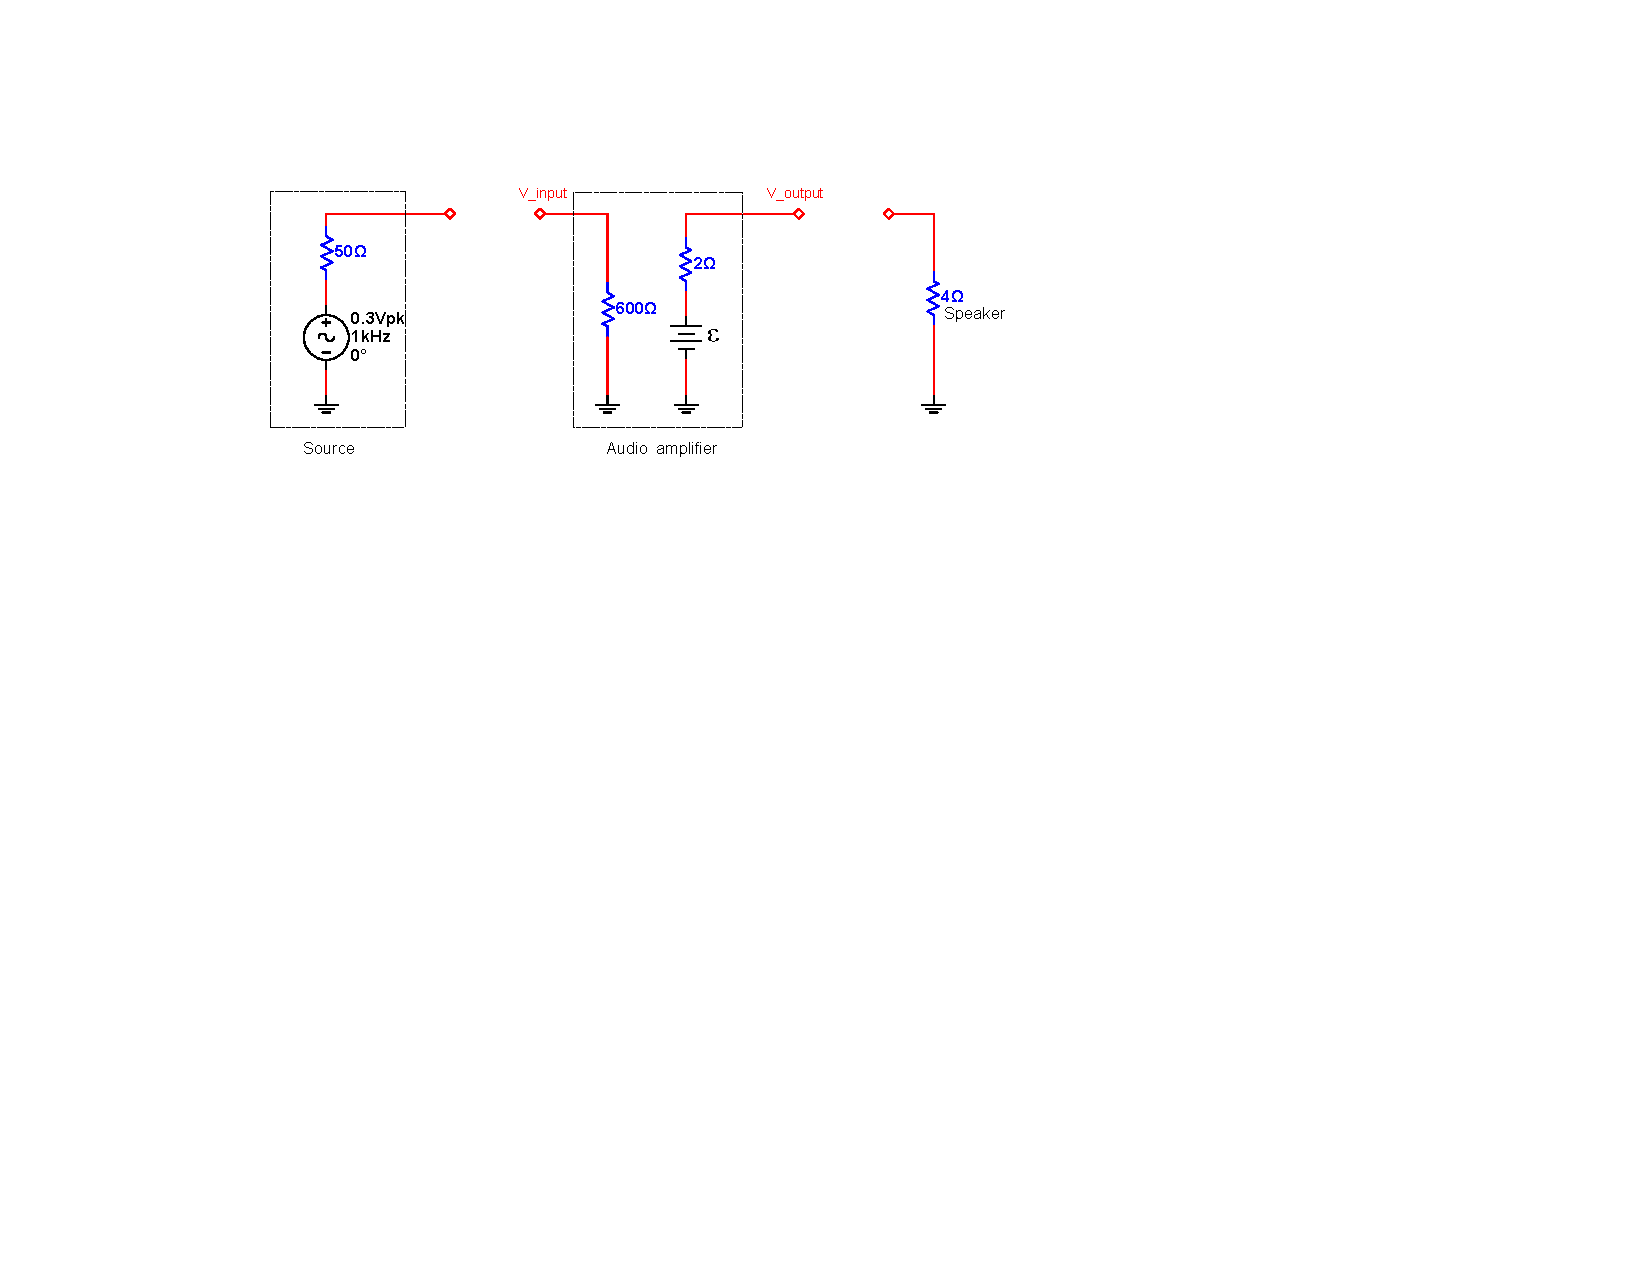
\includegraphics{M_problems/opamps_digital/audio_amplifier.pdf}
\end{center}
\end{Exercise}
\begin{Answer}
(a) 37 V (b) 900 mV
\end{Answer}

%--------------------------------------------------------------------------------------------------------------
\begin{Exercise}
Goofus and Gallant have been learning about op-amps.  Goofus believes that by flipping the $V_+$ and $V_-$ terminals of the op-amp, he has invented a handy way to build a non-inverting summing amplifier, shown below:
\begin{center}
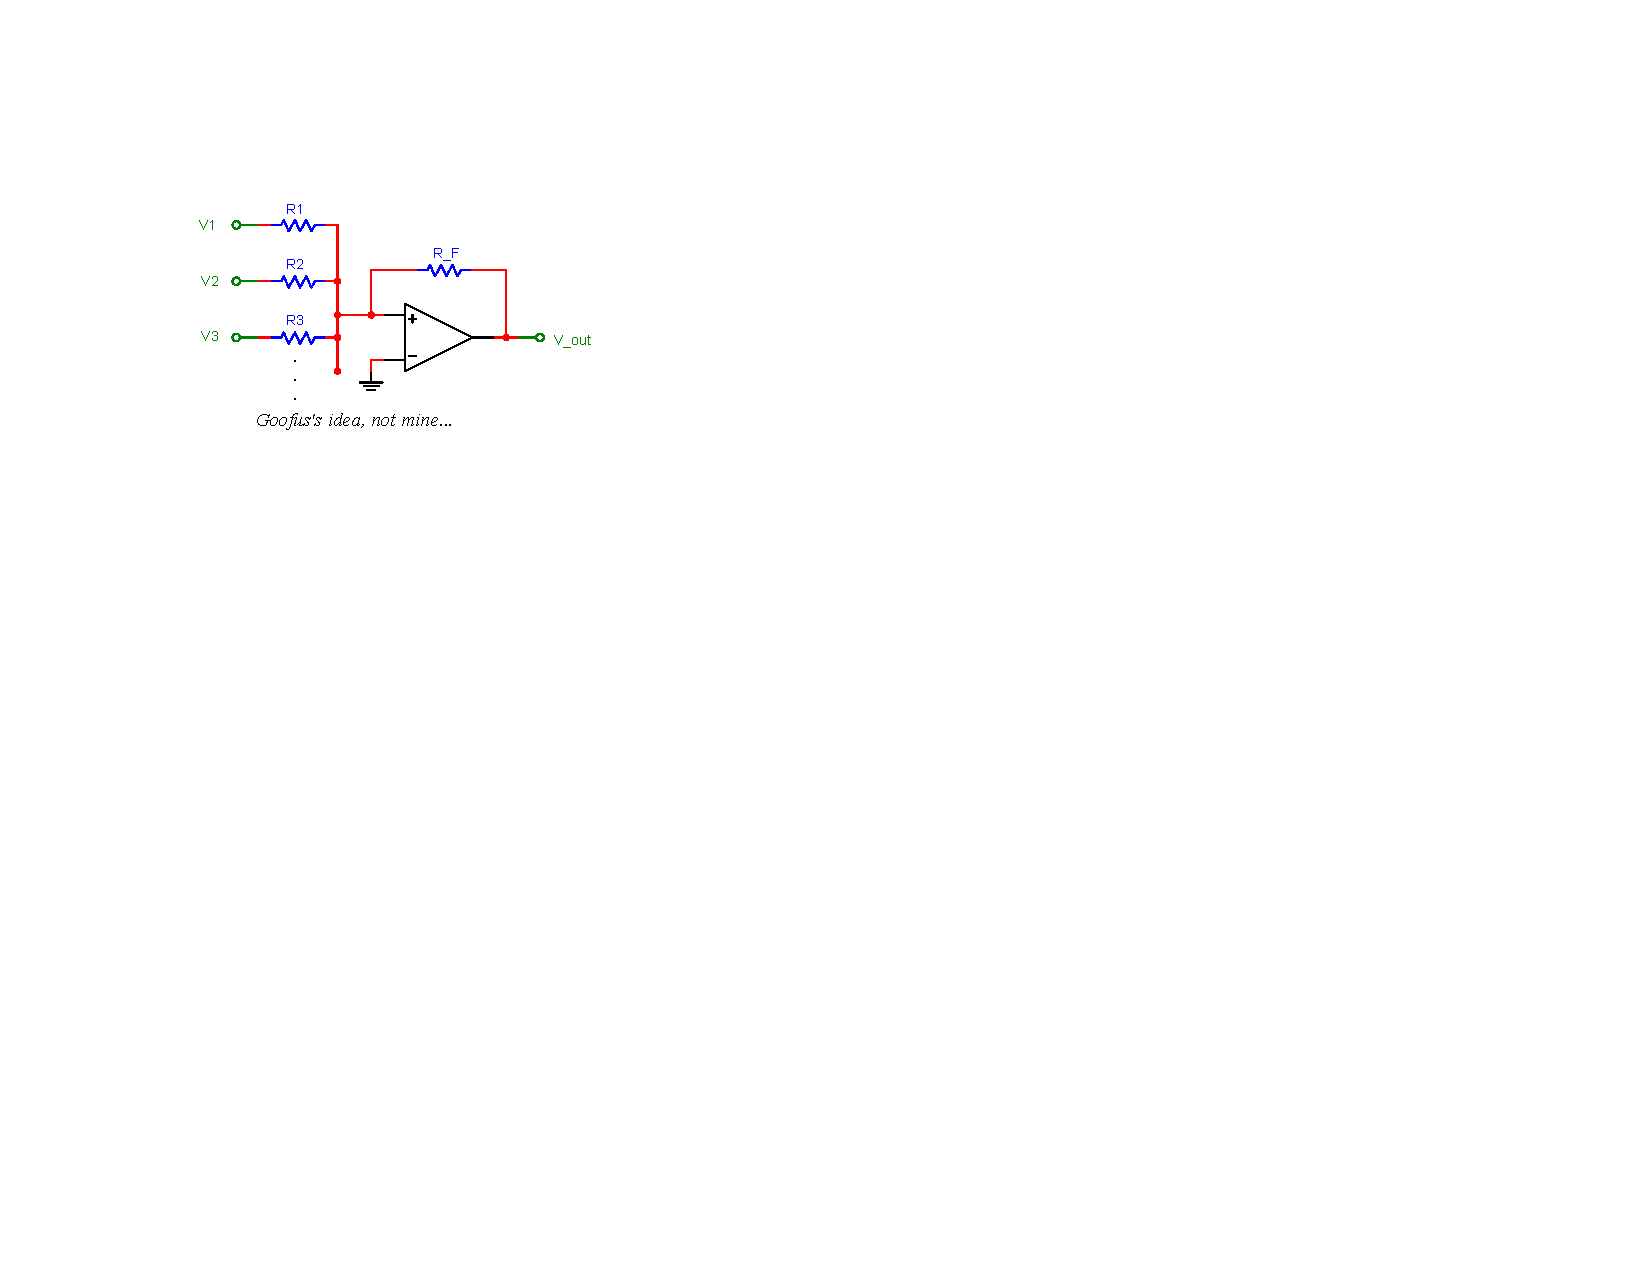
\includegraphics{M_problems/opamps_digital/summing_amp_goofus.pdf}
\end{center}
Goofus explains to Gallant that it should work perfectly, according to the golden rules:
\begin{itemize}[nosep]
\item By Golden Rule 2, $V_+=V_-=0$ volts.
\item By Golden Rule 1, no current flows into the $V_+$ input, so 
$I_{RF}=\dfrac{V_1}{R_1} +  \dfrac{V_2}{R_2}+\dfrac{V_3}{R_3} .$
\item Based on the current through $R_F$, the output should be 
$V_{\rm out}=+R_F \left( \dfrac{V_1}{R_1} +  \dfrac{V_2}{R_2}+\dfrac{V_3}{R_3} \right)$.
\end{itemize}
\vspace{-0.1in}
\begin{enumerate}[label=(\alph*),nosep]
\item Write a short, condescending email from Gallant to Goofus that explains what's wrong with his reasoning.  
\item Include in your email what the output of his circuit would \textit{actually} be were he to build it, \textit{and why}.
\end{enumerate}
\end{Exercise}
\begin{Answer}
Hints:
(a)~Your explanation to Goofus will almost surely involve the words \textit{feedback, negative,} and \textit{positive}.
(b)~The actual output is guaranteed to be either $\approx+15$~V or $\approx-15$~V, pinned at one of the two power rails.  But Goofus won't intuit this on his own, so you still need to explain to him why.
\end{Answer}


%--------------------------------------------------------------------------------------------------------------
\begin{Exercise}
A noninverting amplifier with a gain $G=5$ (as in 
Lab \ref{lab_op-amps} 
part \ref{part_inverting_amplifier}) 
needs to provide an output of 30~mA to a load at $V_{\rm out}=5$~volts.  (That is, the load resistance is $R_{\rm load}=167\ohm$.) 
The maximum output current of the op-amp is 40~mA. 
(a)~What are the minimum values of the two resistors $R_1$ and $R_2$ that could be used, so that they don't draw too much current?  
(b) Why might very large values for the two resistors, like in the range of several $\Mohm$ or more, also cause your circuit to not work correctly? Note: to avoid these two problems, your default should be to pick $R_1$ and $R_2$ (the ``feedback resistors'') in the $10\kohm$ or $100\kohm$ ranges.  If you do that, you don't have to worry about it or calculate anything; it'll mostly just work.
\end{Exercise}
\begin{Answer}
(a) $100\ohm$ and $400\ohm$ (b) Hint: what might be a realistic value for the input impedance of the $V_-$ input?
\end{Answer}

%--------------------------------------------------------------------------------------------------------------
\begin{Exercise}
The circuit below is essentially a differential amplifier, but with unusual values of all four resistors.  It's not obvious what the use of such a circuit would be, but set that aside and use the ``golden rules'' of op-amps to calculate 
(a)~the voltages at the inputs $V_+$ and $V_-$, 
(b)~the output voltage $V_{\rm out}$, and 
(c)~the output current of the op-amp.  (That is, the current coming out of the output pin of the op-amp, not necessarily the current in the load resistor.)  
\begin{center}
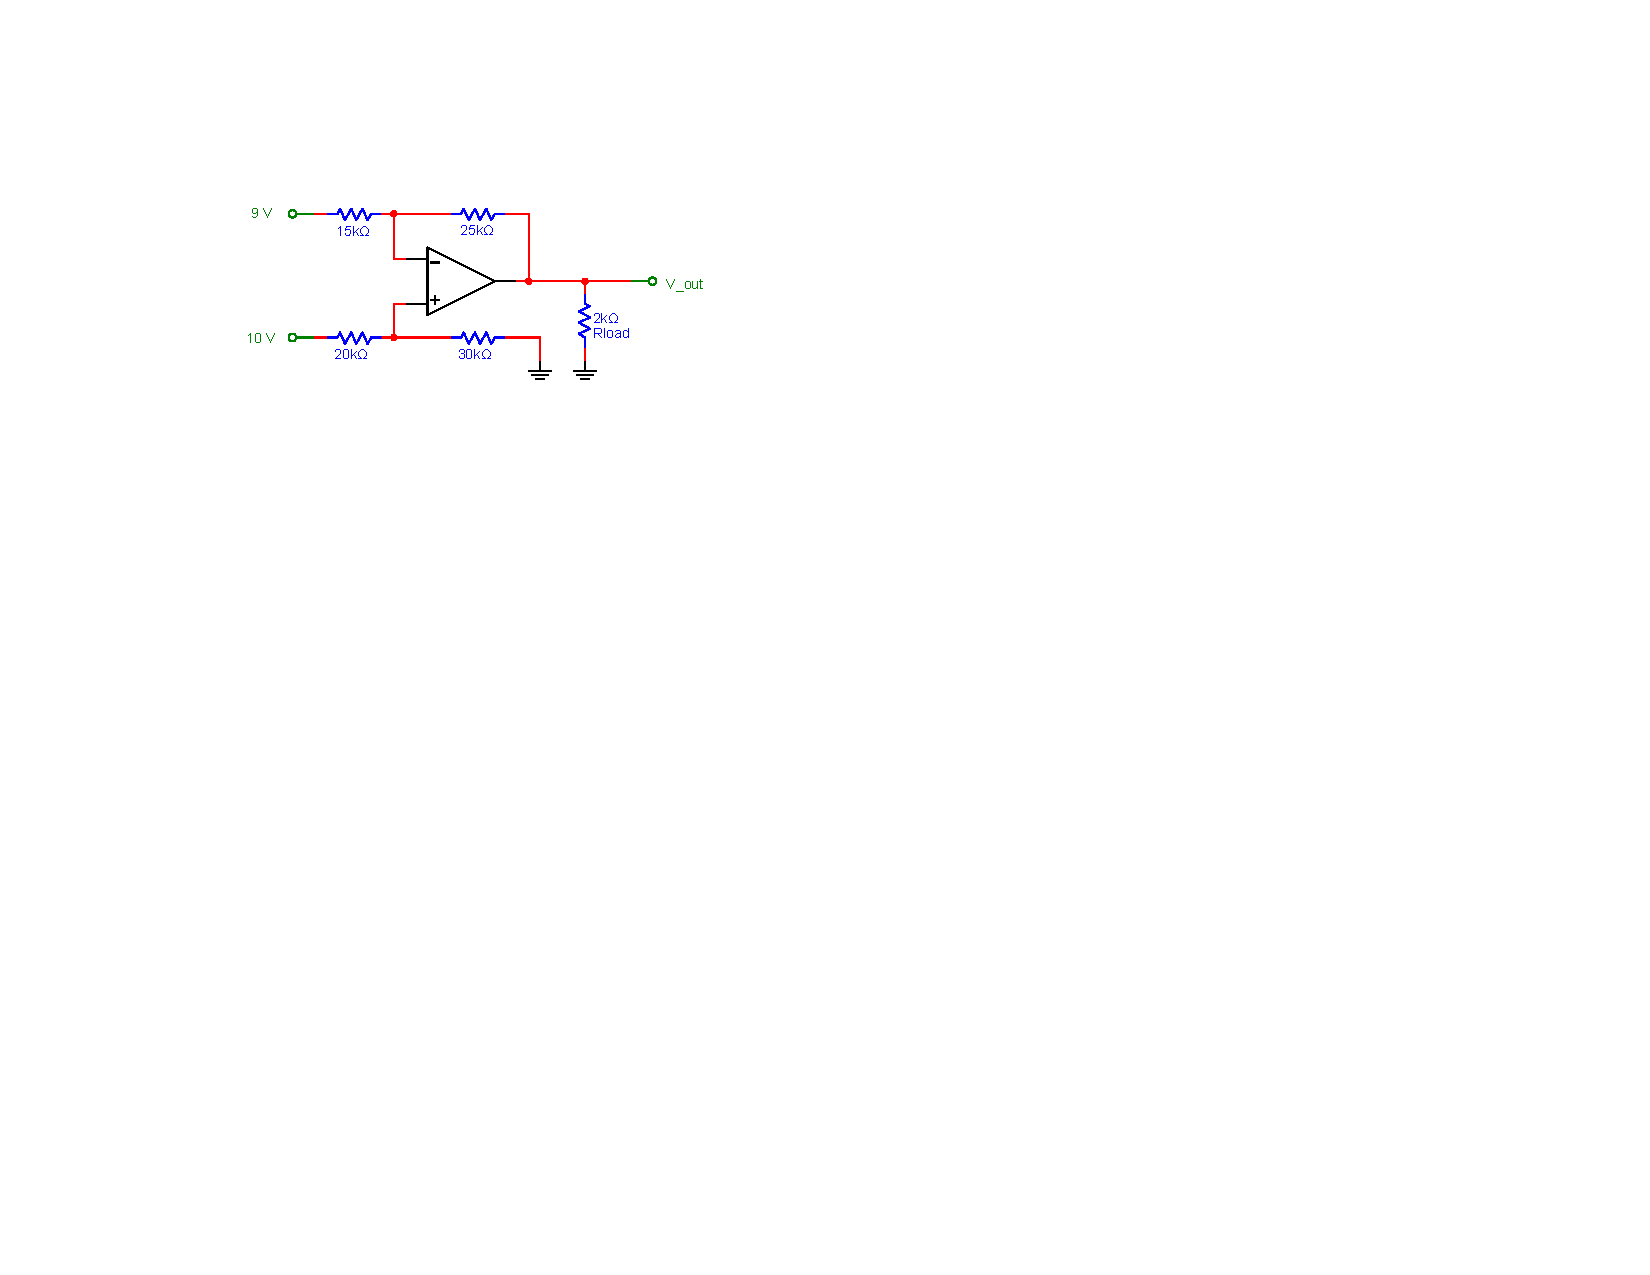
\includegraphics{M_problems/opamps_digital/differential_amp_odd.pdf}
\end{center}
\end{Exercise}
\begin{Answer}
(a)  $V_+=V_-=6$ volts  (b) 1 volt (c) 300 $\mu$A
\end{Answer}

%--------------------------------------------------------------------------------------------------------------
\begin{Exercise}
On page 749 of our textbook by Paynter, the author relates an op-amp's maximum usable frequency to its slew rate by plunking down Equation 22.5,
$$f_{\rm max}=\frac{{\rm slew~rate}}{2\pi V_{\rm pk}},$$
with no explanation of where it might come from or why it might be true.  Derive this equation, providing the explanation that Paynter left out.  Incidentally, the lack of motivation for equations like this is one of the reasons I'm not crazy about this book.  I suspect it stems in part from the assumption that the readers' math ability is so exceptionally low that they are just \textit{barely} able to plug numbers into a formula that's provided for them, laboriously pressing the calculator buttons with their knuckle pads and then requiring a long rest. 
\end{Exercise}


%Ideas for additional problems:

\vspace{0.75in plus 0.75in minus 0.2in} 

%\pagebreak[3]
\textbf{Answers to Selected {\thesubsection} Problems:}
\label{opamps_digital_prob_answers}
%\shipoutExercise
\shipoutAnswer

\cleardoublepage


\begingroup
	%The next subsection is hardwired to be ``i'' as in (-1)^(1/2).  Afterwards, the counter is decrimented to resume where it had been.
	\renewcommand{\thesubsection}{\thesection\textit{i}}
	\subsection{Complex Numbers} 

%\DTMnewdatestyle{dateupdated}{〈definition 〉

Answers to \thesubsection ~problems are on page \pageref{complex_numbers_answers}.  \textbf{\textcolor{red}{Updated \DTMnow.}}

%--------------------------------------------------------------------------------------------------------------
\begin{Exercise}
Find the real and imaginary parts of $4i - 3$.
\end{Exercise}
\begin{Answer}
4 and $-3$, respectively
\end{Answer}

%--------------------------------------------------------------------------------------------------------------
\begin{Exercise}
Find the magnitude (aka ``modulus'' or ``absolute value'') of $4-3i$.
\end{Exercise}
\begin{Answer}
5
\end{Answer}

%--------------------------------------------------------------------------------------------------------------
\begin{Exercise}
Find the phase (aka ``argument'') of $4+3i$.
\end{Exercise}
\begin{Answer}
0.643
\end{Answer}

%--------------------------------------------------------------------------------------------------------------
\begin{Exercise}
Find the phase of (a) $-4+3i$ and (b) $-4-3i$.  (Hint: your calculator lies.  Graph it.)
\end{Exercise}
\begin{Answer}
(a) 2.50 (b) 3.78 or $-2.50$
\end{Answer}

%--------------------------------------------------------------------------------------------------------------
\begin{Exercise}
Find the real and imaginary parts of $6e^{i \pi/6}$.
\end{Exercise}
\begin{Answer}
5.20 and 3, respectively
\end{Answer}

%--------------------------------------------------------------------------------------------------------------
\begin{Exercise}
Find the magnitude and phase of $6e^{i(4\pi /7)}$.
\end{Exercise}
\begin{Answer}
6 and $4\pi / 7$
\end{Answer}

%--------------------------------------------------------------------------------------------------------------
\begin{Exercise}
Find the real and imaginary parts of $(3+2i)(-4-6i)$.
\end{Exercise}
\begin{Answer}
0 and $-26$
\end{Answer}

%--------------------------------------------------------------------------------------------------------------
\begin{Exercise}
Find the real and imaginary parts of $(2+3i)/(4-5i)$.  (Hint: multiply both the numerator and denominator by the denominator's complex conjugate.)
\end{Exercise}
\begin{Answer}
$-0.1707$ and 0.537
\end{Answer}

%--------------------------------------------------------------------------------------------------------------
\begin{Exercise}
Plot each of the following on the complex plane: $e^{i\cdot 0}$, $e^{i\pi /2}$, $e^{i\pi}$, and $e^{i ∙3\pi / 2}$.
\end{Exercise}
\begin{Answer}
Your points are the same as $1, i, -1$, and $-i$.
\end{Answer}

%--------------------------------------------------------------------------------------------------------------
\begin{Exercise}
Write $4+3i$ in the form $re^{i\theta}$.
\end{Exercise}
\begin{Answer}
$5e^{0.643i}$
\end{Answer}

%--------------------------------------------------------------------------------------------------------------
\begin{Exercise}
What are the magnitude and phase of $e^{i\pi/6} e^{i\pi/4}$?
\end{Exercise}
\begin{Answer}
1 and $5\pi/12$
\end{Answer}

%--------------------------------------------------------------------------------------------------------------
\begin{Exercise}
What are the magnitude and phase of $(4+3i) e^{0.2i}$?
\end{Exercise}
\begin{Answer}
5 and 0.843
\end{Answer}

%--------------------------------------------------------------------------------------------------------------
\begin{Exercise}
Suppose $f(t)= 20e^{i\omega t}$, where $\omega=5$~sec$^{-1}$.  Find the magnitude and phase of $f(t)$ at (a)~$t=0$~seconds and (b)~at $t=0.27$~seconds.
\end{Exercise}
\begin{Answer}
(a) 20 and 0 (b) 20 and 1.35
\end{Answer}

%--------------------------------------------------------------------------------------------------------------
\begin{Exercise}
Suppose $f(t)= (6+8i) e^{i\omega t}$, where $\omega=5$~sec$^{-1}$.  Find the magnitude and phase of $f(t)$ at (a)~$t=0$~seconds and (b)~at $t=0.27$~seconds.
\end{Exercise}
\begin{Answer}
(a) 10 and 0.927 (b) 10 and 2.277 
\end{Answer}

%--------------------------------------------------------------------------------------------------------------
\begin{Exercise}
The ``exponential rule'' for derivatives of exponential functions is that $\displaystyle \frac{d}{dx} e^u=e^u  \frac{du}{dx}$.  
Show by direct substitution of the Euler formula, $e^{i \theta}=\cos \theta + i \sin \theta$, that the exponential rule yields the correct results for  $\displaystyle \frac{d}{dt} (Ae^{i\omega t}) \text{~and~}  \frac{d}{dt}(Ae^{-i\omega t})$.
\end{Exercise}




%\newcommand{\figuretoright}{3} {%
	%#1 is the picture width
	%#2 is the text to the right



%Ideas for additional problems:

%\vfill

\vspace{2in}

\pagebreak[3]

\textbf{Answers to Selected {\thesubsection} Problems:}
\label{complex_numbers_answers}
%\shipoutExercise
\shipoutAnswer

\cleardoublepage

	\addtocounter{subsection}{-1}
\endgroup

\subsection{Capacitors, Inductors, and AC circuits} 

%\DTMnewdatestyle{dateupdated}{〈definition 〉

Answers to M\Alph{subsection} problems are on page \pageref{C_L_and_AC_prob_answers}.  \textbf{\textcolor{red}{Updated \DTMnow.}}

%--------------------------------------------------------------------------------------------------------------
\begin{Exercise}
A 200 nF capacitor is charged by a 5~V supply through a $2\kohm$ resistor, starting at zero volts.  (a)~Graph both the current $I_C$ through the capacitor and the voltage $V_C$ across the capacitor as functions of time.  (b)~At what time does the capacitor voltage reach 90\% of the supply voltage?  (c)~What is the current through the resistor at the time you calculated in part (b)?
\end{Exercise}
\begin{Answer}
(b) $921~\mu$sec (c) $250~\mu$A
\end{Answer}

%--------------------------------------------------------------------------------------------------------------
\begin{minipage}{0.7\textwidth}
\begin{Exercise}
A student wants to find the internal resistance of a standard, size-AA battery.  With no load resistor connected, the voltage across the terminals of the battery is 1.55~V.  But when the battery is connected to a load resistor of 10~$\Omega$ (as shown on the right) the voltage across the load resistor is 1.47~V.  What is the internal resistance of the battery?
\end{Exercise}
\begin{Answer}
0.544~$\Omega$ The circuit is built correctly and the output is within the range expected for the tolerances of the components. The circuit is built correctly and the output is within the range expected for the tolerances of the components. The circuit is built correctly and the output is within the range expected for the tolerances of the components.
\end{Answer}
\end{minipage}
\begin{minipage}{0.30\textwidth - 5pt}
\hfill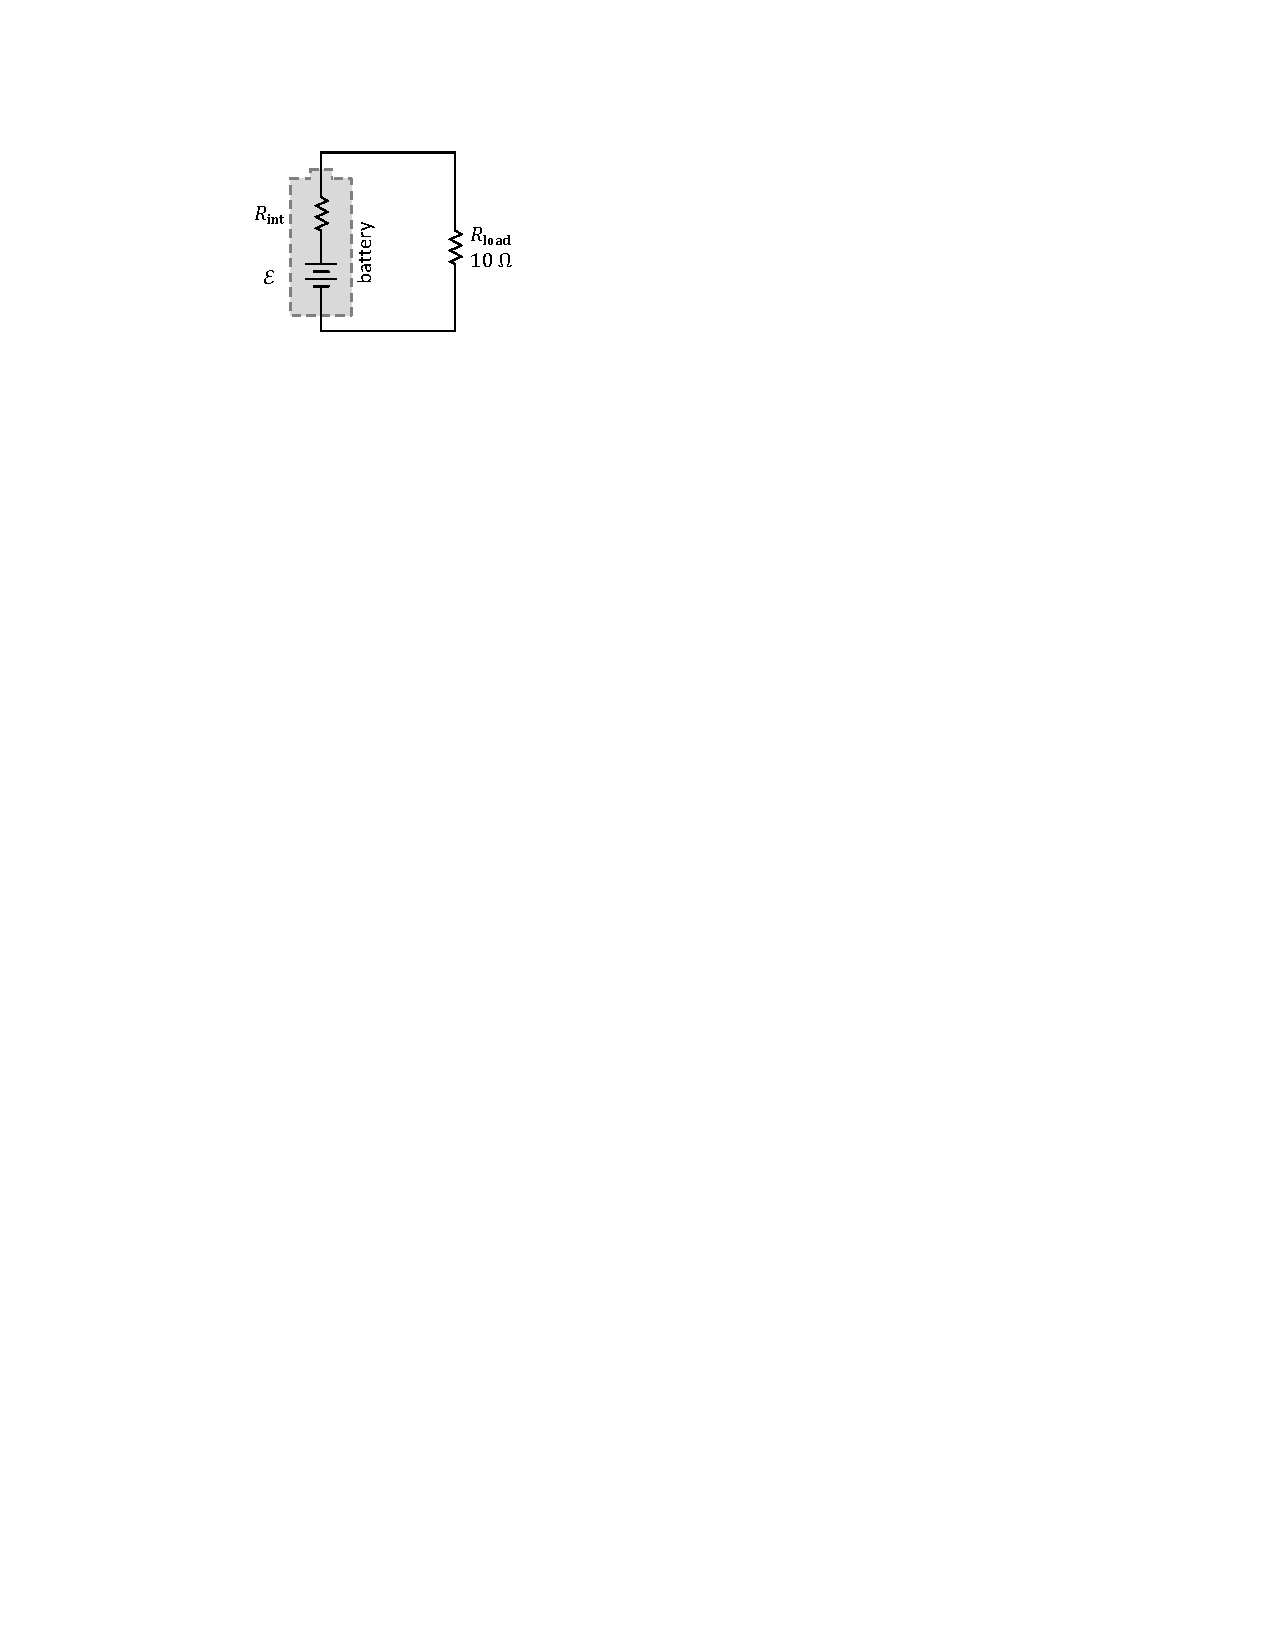
\includegraphics{M_problems/the_basics/real_battery_10ohms.pdf}
\end{minipage}

%--------------------------------------------------------------------------------------------------------------
\begin{Exercise}
The figures below show two possible circuits you could use to measure the current and voltage of a resistor.  Both methods are imperfect, due to the non-ideal input impedances of the voltmeter and the ammeter.  
(a)~Which circuit will give a current reading that is slightly inaccurate, due to the non-ideal voltmeter?  
(b)~Will that current reading be too high or too low?  
(c)~Which circuit will give a voltage reading that is slightly inaccurate, due to the non-ideal ammeter?  
(d)~Will that voltage reading be too high or too low? 
(e)~Suppose the impedances of the two meters are $10\ohm$ and $10\Mohm$.  Which circuit is preferable if the resistor you are measuring has $R=100\ohm$, and why?  (f) Which circuit is preferable if the resistor you are measuring has $R=1\Mohm$, and why?
\begin{center}
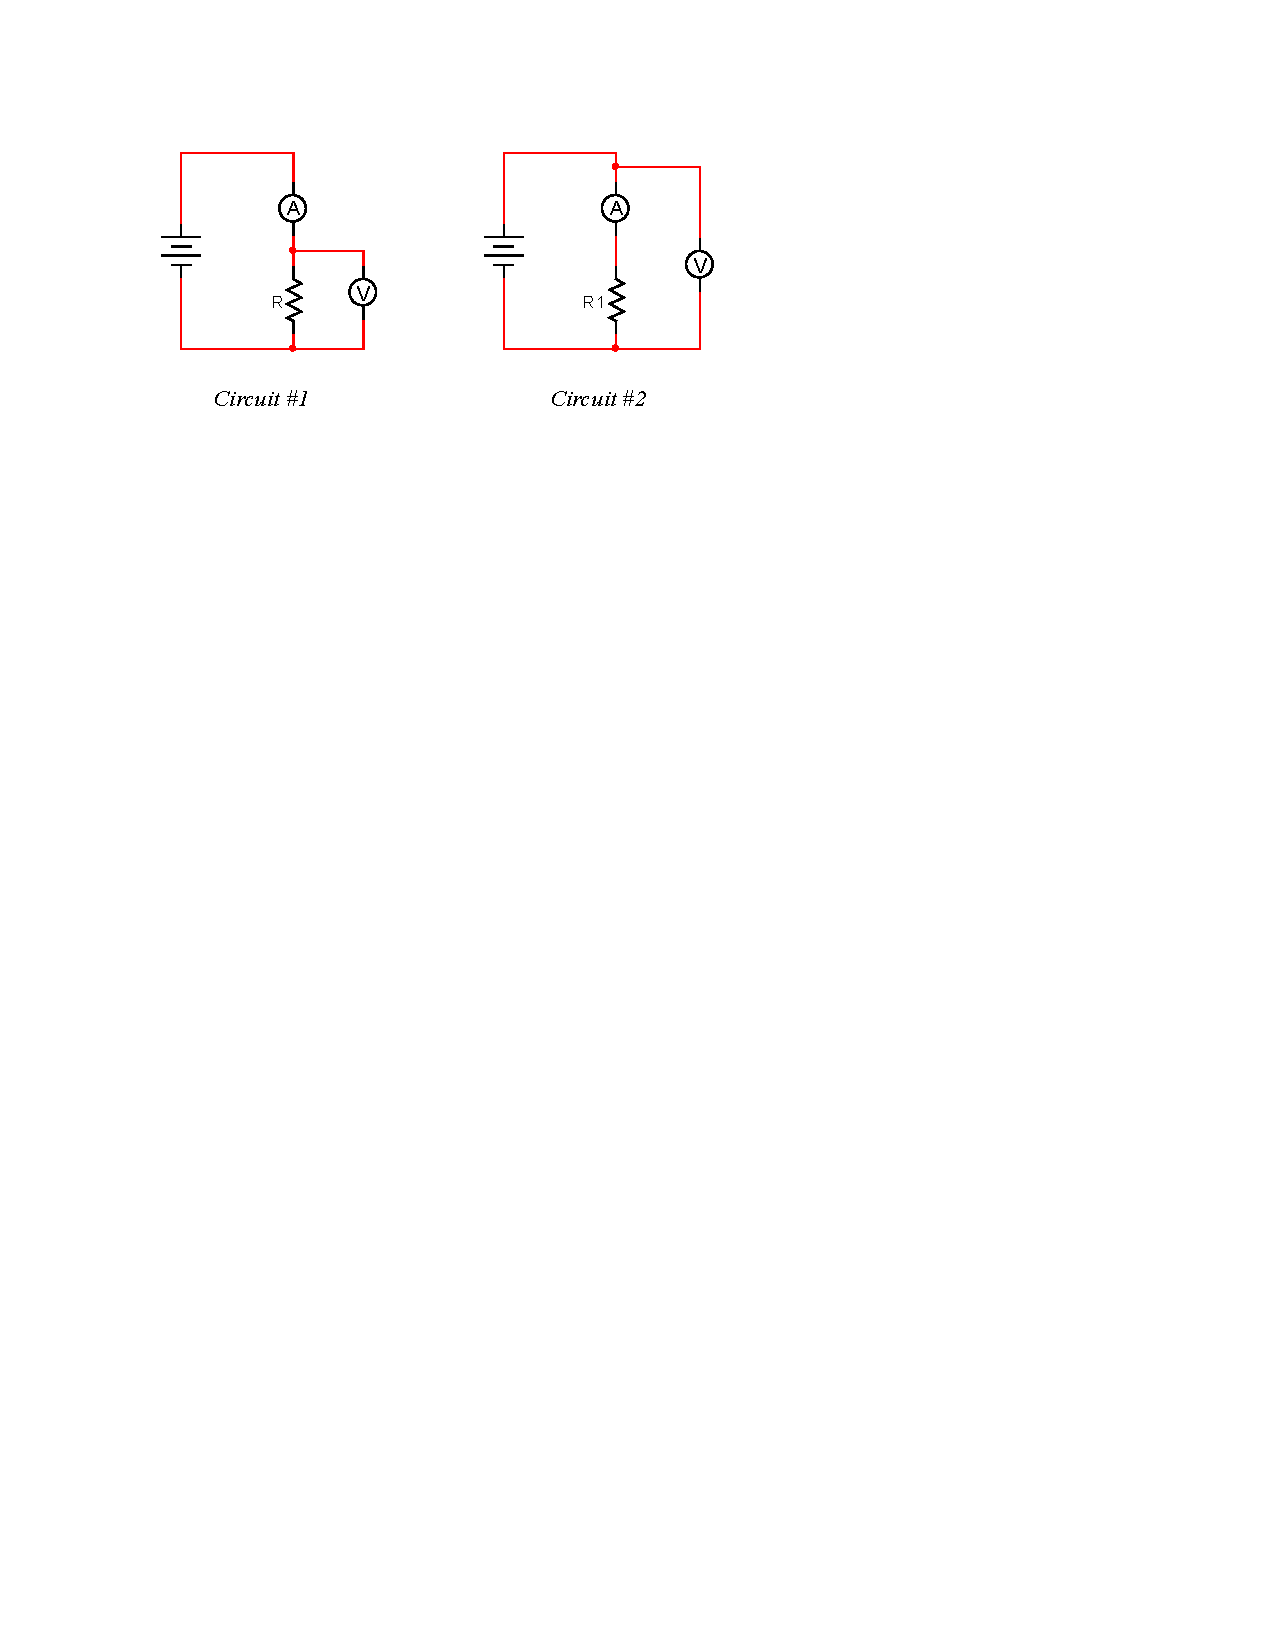
\includegraphics{M_problems/the_basics/I_V_measurements.pdf}
\index{color page}
\end{center}
\end{Exercise}
\begin{Answer}
(a) circuit \#1 (c) circuit \#2 (d) too high (e) circuit \#1
\end{Answer}

%\newcommand{\figuretoright}{3} {%
	%#1 is the picture width
	%#2 is the text to the right



%Ideas for additional problems:

%\vfill
%\pagebreak[3]

\vspace{0.7in}

\textbf{Answers to Selected {\thesubsection} Problems:}
\label{C_L_and_AC_prob_answers}
%\shipoutExercise
\shipoutAnswer

\cleardoublepage

